%%
%%  Department of Electrical, Electronic and Computer Engineering.
%%  EPR400/2 Final Report - Main File.
%%  Copyright (C) 2011-2018 University of Pretoria.
%%

\documentclass{epr400}

\usepackage{ragged2e}

\usepackage{algorithmic}
%\usepackage[ruled,linesnumbered]{algorithm2e}
%\usepackage{algpseudocode}


%\usepackage[font={small}]{caption}

%% EDIT: Replace the following with your information.
\eprtitle{Design of an electonic home shopping list}
\eprcode{EPR402}
\eprcandidatename{J.K. Mahlokozela}
\eprstudentnumber{15145574}
\eprdate{November 2018}
\eprsupervisor{Prof T. Stander}

\hyphenpenalty=10000
\allowdisplaybreaks


\begin{document}

%% Generate the required title page.
\begin{flushleft}
\maketitlepage
\end{flushleft}


%% --- PART 1 ------------------------------------------------------------

\pagestyle{plain}
\pagenumbering{roman}

\eprsec{Part 1. Preamble}

\vspace*{0.5cm}

%% Import the required preamble pages.
%%
%%  Department of Electrical, Electronic and Computer Engineering.
%%  EPR400/2 Final Report - Preamble.
%%  Copyright (C) 2011-2018 University of Pretoria.
%%

This document is a report showing the work that I did in designing a home shopping list device. The device was designed using data structures and algorithms as well as digitally communicating components.
\\[2ex]
\textit{Project proposal and technical documentation} \newline
A copy of the approved Project Proposal is contained in Part 3 of this report and technical documentation is also included in Part 5 of the report. The technical section of the report documents the hardware schematics and the software code implemented. This appendix is included on a CD that accompanies the report.
\\[2ex]
\textit{Project history} \newline
The work done by Srihari (2000) in implementing learning dependent optical character recognition is an important foundation of this project. The hardware was provided by the Adafruit Industries. Some of the functions in the algorithm associated with handwriting recognition was adapted from Shiffman (2010). The rest of the work documented in this report was my own.
\\[2ex]
\textit{Language editing} \newline
This document has been language edited by a knowledgeable person. By submitting this document in its present form, I declare that this is the written material that I wish to be examined on.

My language editor was \underline{    Mr Bernard Mazimbo    }

% \makebox[3in]{\hrulefill}.

\vspace*{0.5cm}

\begin{tabular}{lp{1cm}ll}
\makebox[3in]{\hrulefill}  &  & \makebox[1.5in]{\hrulefill} \\
\textit{Language editor signature}  &  & \textit{Date}
\end{tabular}

\vspace*{0.5cm}

\textit{Declaration}
\\[2ex]
%I, \makebox[3in]{\hrulefill} understand what 
I, \underline{  Joe Kumbirai Mahlokozela  } understand that
plagiarism is and have carefully
studied the plagiarism policy of the University. I hereby declare that all the
work described in this report is my own, except where explicitly indicated
otherwise. Although I may have discussed the design and investigation with my
study leader, fellow students or consulted various books, articles or the
Internet, the design/investigative work is my own. I have mastered the design
and I have made all the required calculations in my lab book (and/or they are
reflected in this report) to authenticate this. I am not presenting a complete
solution of someone else.

Wherever I have used information from other sources, I have given credit by
proper and complete referencing of the source material so that it can be
clearly discerned what is my own work and what was quoted from other sources.
I acknowledge that failure to comply with the instructions regarding
referencing will be regarded as plagiarism.  If there is any doubt about the
authenticity of my work, I am willing to attend an oral ancillary
examination/evaluation about the work.

I certify that the Project Proposal appearing as the Introduction section of
the report is a verbatim copy of the approved Project Proposal.

\begin{tabular}{lp{1cm}ll}
\makebox[3in]{\hrulefill}  &  & \makebox[1.5in]{\hrulefill} \\
\eprthecandidatename       &  & Date
\end{tabular}

%% End of File.


\newpage

%% Add the Table of Contents.
\tableofcontents
\thispagestyle{empty}
\newpage

%% Import the required abbreviation pages.
%%
%%  Department of Electrical, Electronic and Computer Engineering.
%%  EPR400/2 Final Report - Abbreviations.
%%  Copyright (C) 2011-2018 University of Pretoria.
%%

\section*{LIST OF ABBREVIATIONS}

\begin{tabular}{p{3cm}l}
%  \textbf{AWGN}         &  Additive white Gaussian noise \\
%  \textbf{BER}          &  Bit error rate \\
%  \textbf{BPSK}         &  Bipolar phase shift keying \\
%  \textbf{DSP}          &  Digital signal processor \\
%  \textbf{GSM}          &  Global System for Mobile communications \\
%  \textbf{SNR}          &  Signal-to-noise-ratio  \\
\textbf{LAN}		& Local Area Network \\
\textbf{HMI}		& Human-Machine Interface\\
\textbf{PC}			& Personal Computer\\
\textbf{LRM}		& Linear Regression Model\\
\textbf{PCB}		& Printed Circuit Board \\
\textbf{WAN}		& Wide Area Network\\
\textbf{WLAN}		& Wireless Local Area Network\\
\textbf{ASCII}		& American Standard Code for Information Interchange\\
\textbf{IDE}		& Integrated Development Environment\\
\textbf{OCR}		& Optical Character Recognition\\
\textbf{BER}		& Bit error rate\\
\textbf{BPSK}		& Bipolar phase shift keying\\
\textbf{DSP}		& Digital signal processor\\
\textbf{CPU}		& Central Processing Unit\\
\textbf{CNS}		& Central Nervous System\\
\textbf{GSM}		& Global System for Mobile communications\\
\textbf{SNR}		& Signal-to-noise-ratio\\ 
\textbf{RPi}		& Raspberry Pi\\
\textbf{OS}			& Operating System\\
\textbf{FDMA}		& Frequency Division Multiple Access \\
\textbf{ISDN}		& Integrated Services Digital Network \\
 \textbf{PLMN}		& Public Land Mobile Network \\
 \textbf{CC}		& Country Code \\
\textbf{SN}			& Subscriber Number \\
\textbf{NDC}		& National Destination Code\\ 
\textbf{ME}			& Mobile Equipment \\
\textbf{SIM}		& Subscriber Identity Module\\ 
\textbf{PUK}		& Personal Unblocking Key\\
\textbf{IBSS}		& Independent Basic Service Set\\ 
\textbf{STA}		& Station \\
\textbf{BSS}		& Basic Service Set \\
\textbf{ESS}		& Extended Service Set \\
\textbf{NIC}		& Network Interface Card \\
\textbf{DS}			& Direct Sequence \\
\textbf{AES}		& Advanced Encryption Standard \\
\textbf{RNN}		& Recurrent Neural Network\\
\textbf{GUI}		& Graphical User Interface\\
\end{tabular}

%% End of File.

\newpage

%% --- PART 2 ------------------------------------------------------------

\eprsec{Part 2. Summary}

%% Import the summary section
%%
%%  Department of Electrical, Electronic and Computer Engineering.
%%  EPR400/2 Final Report - Section 2.
%%  Copyright (C) 2011-2018 University of Pretoria.
%%

This report describes the work that was done in developing a home shopping list device. The aim of the device was to recognize shopping list data in the form of handwriting input, convert it to text and save it. The device would then send the converted shopping list data to the user’s phone when they requested it. 

\textbf{What has been done}
%(Add a figure or figures here – this will probably be a figure that also appears in section 4 of the report).

A literature study was conducted and completed on different handwriting recognition schemes. The literature study also overreached to include designs that are used in modern communication systems. The software for the handwriting recognition system of the device was developed from first principles. The integral component of the system is a Raspberry Pi board. The rest of the hardware, mostly off the shelf was connected to this RPi board. A Python program was used to simulate the recognition process on a Linux OS. The communication process was also simulated using a Python program. A Wi-Fi connection was programmed onto the integral Raspberry Pi board. These programs were then integrated to work concurrently and then implemented onto the Raspberry Pi board.

What has been achieved
The device developed produced was able to successfully send the shopping list written by the user to their phone on request. The test case distance for the communication was 40 km. The device also converted the handwritten shopping list data to readable text at an acceptable error level. Higher accuracy levels could be implemented by training the recognition algorithm with the already converted shopping list data, but the trade-off was that it would take too long to convert the  
input thereby inconveniencing customers. 


\textbf{Findings}

A discovery that was made during the design and implementation of the device was that the number of hidden layers used in the recognition algorithm’s neural network affected the accuracy of the recognition scheme. More hidden layers generally increased the accuracy of the scheme. The number of hidden layers also impacted the time taken to convert the input to readable text. More hidden layers led to more time taken for full conversion. Therefore, the number of hidden layers had to be designed carefully to consider the trade-off of optimizing accuracy as well as minimizing conversion time.

\textbf{Contribution}

Code was mostly developed by the student, with a strong reliance on existing libraries. As the code was of large scope, some modules were taken directly from existing libraries, while other modules were coded from first principles. Friends in class initially helped with coding in R for statistical analyses, as this was complex and completely new to the student.

Programming of the Graphical User Interface was done by using PyQt. The student had minor familiarity with Qt, a C++ equivalent of PyQt. Therefore, the theory associated with programming in the PyQt development environment was first mastered and the user interface was developed afterwards. The geometry bounds associated with the development environment were important in the design section to be explored later. 

SSL communication was mastered for the device’s communication system to be successfully implemented. The student had no familiarity with the Basic “AT” commands associated with communication, so a thorough understanding was established from Mouly (1996). The student then developed the code for the communication of the home shopping list device and the student’s cell phone. This code was developed in Python. 

The recognition algorithm was implemented using the IDE software called Spyder3. Spyder3 uses the Python programming language. There was some mild familiarity with Python as the language was earlier used for simulating non-complex digital signal processing. Complex Python programming was studied from Rollins (2006). No assistance was required from the study leader when the code was initially implemented. Once the software was integrated onto the hardware, the study leader’s feedback was collected, and the software was tweaked as specified. The study leader was mostly helpful with complications in hardware integration.


\newpage

%% End of File.



%% --- PART 3 ------------------------------------------------------------

\eprsec{Part 3. Project identification: approved Project Proposal}

%% Import the approved project proposal
%%
%%  Department of Electrical, Electronic and Computer Engineering.
%%  EPR400/2 Final Report - Proposal.
%%  Copyright (C) 2011-2016 University of Pretoria.
%%

This section contains the problem identification in the form of the complete
approved Project Proposal, unchanged from the final approved version.

\newpage

% Reset the section counter
\setcounter{section}{0}



%\import{proposal}

{
%\let\stdthebibliography\thebibliography
%\renewcommand{\thebibliography}{%
%  \let\section\subsection
%  \stdthebibliography}
%\begin{bibunit}[IEEEtran]

%\section{Problem statement}
%%
%%  Department of Electrical, Electronic and Computer Engineering.
%%  EPR400/2 Project Proposal - Section 1.
%%  Copyright (C) 2011-2018 University of Pretoria.
%%

\section{Problem statement}

\textbf{Motivation} \\
Shopping is a common chore for the average household\cite{Block:Shopping}. Before going shopping, a customer has to take note and write down their shopping list items one at a time, on a piece of paper. The customer then has to carry the shopping list everywhere they go, in case they need to do their shopping. The problem associated with this is that, since the list is written on a piece of paper, it is prone to being lost or forgotten at home, which leads to inconveniences when the customer wants to do their shopping. %A device has to be developed to account for t
%The present method of gathering shopping lists does not seem to be moving with the times of evolving technological advancements and is not secure from misplacing. Therefore the problem to be taken care of is to develop a system that is more efficient in how it assists users with gathering their shopping lists.
\noindent
\\\\
\textbf{Context} \\
%Everyone needs to do their shopping once in a while.
%A device should be produced as the end-product to the customer. The device shall be able to assist the customer with their shopping. The customer writes their shopping list on the device while at home and the list is automatically saved within the device, while the customer is writing the list. When the customer is shopping and realizes that they need the list, it should be sent to them, at the click a button that requests the list.
The best methods of solving a problem like this involve integration of home-based automation systems and control systems\cite{Kuo:Automatic_Control_Systems}, with devices being controlled by instructions from the user\cite{Yuksekkaya:Automation_Systems}.
%The customer currently writes their shopping list on a piece of paper, one item after another. The customer then has to carry the shopping list everywhere they go, in case they need to do their shopping. Since the list is written on a piece of paper, it will be prone to being lost, which is a major inconvenience.
A solution that has been tried before to ensure that lists do not get lost, is that of saving a screenshot of the customer's list, on their phone\cite{WinNT}. This solution is not desirable due to the fact that the customer cannot then cross things off their list if they change their mind. Another solution currently in use is that of using the Android application called "ShopList"\cite{ShopL}. The biggest drawback is that it is not flexible enough to add items which are not recognized internally by the program. In addition, the shopping list items can only be recorded by the phone's owner, not other members of the household.\\
The device to be produced to address the problem statement will be a great improvement on these methods because the customer can add any items of their choice to the shopping list and will be able to edit the list as they please. In addition to what has been mentioned, unlike the piece of paper where the shopping list is commonly  written on, the device will be attached to the customer's fridge with no chance of being lost. Also, the customer will not have to worry about losing their shopping list because it will always be with them at the tip of a button on their smartphone. The device to be produced also provides the functionality for other members of the household to add items onto the shopping list, unlike shopping applications like ShopList\cite{ShopL}.
\noindent
\\\\
\textbf{Technical Challenge} \\
% engineering challenge is to design and develop a device that takes the customer's shopping list input in handwritten form and saves it so that when the customer requires it, they will only have to press a button on their phone, and the device will send it to them. The engineering aspects of the project are as follows:
The engineering challenges associated with the project are to: (i) develop a small device that operates on a nonchargeable battery power supply, (ii) design and implement a text recognition algorithm to scan the user's input and convert it to recognizable text, (iii) design and implement a communication protocol to enable the device to send messages to the customer's smartphone wherever they are and (iv) design a mobile application that enables the user to obtain their shopping list from the device at home by clicking a single button. \\\\
\noindent
\textbf{Limitations}\\
The mobile application to be used to obtain the shopping list will run on smartphones using the Android Operating System only. Furthermore, the accuracy of the handwriting recognition software will be limited by the Optical Character Recognition code and the neural networks developed for that specific code. Since the customized micro-electronic components cannot be prototyped, the developer will be limited to use low cost components to build the system.
\nocite{Haykin:Communication_Systems}

%% End of File.

%%
%%  Department of Electrical, Electronic and Computer Engineering.
%%  EPR400/2 Project Proposal - Section 2.
%%  Copyright (C) 2011-2018 University of Pretoria.
%%

\section{Project requirements}

\subsection{Mission requirements of the product}
Specific details of the mission requirements of the product are listed below.
\begin{itemize}
	\item The user should get their shopping list sent to their phone from the device when they request for it.
	\item A small portable device must be produced.
	\item The device should run on non-rechargeable batteries.
	\item The device should contain a battery meter and should warn the user when the battery is low.
	\item The produced device must scan input from a user's handwriting and convert it to recognizable text.
	\item The device should display the list in recognizable and readable font.
	\item The produced device must automatically save what is written on its screen, in case the battery dies out.
	\item The user should use a touch-pen to write their shopping list items onto the touchscreen, which saves them into the device's memory.
\end{itemize}
\subsection{Student tasks}
The steps listed below need to be taken for mission requirements to be met.
\begin{itemize}
	\item A program must be developed for a smartphone so that it can request a document from the produced device.
	\item A communication interface must be established between the user's smartphone and the produced device.
	\item A handwriting recognition system must be implemented for conversion from user handwriting to recognizable text. 
	\item A magnetic casing should be designed for the device so that it can be attached to a fridge.
	%\item A program must be developed to capture the information from the touchscreen, either screen-shot capture or text capture.
	\item A polling and timing algorithm should be implemented so that after a specific amount of time, the contents on the touchscreen are automatically saved.
\end{itemize}
\newpage

\newpage

%% End of File.




%%
%%  Department of Electrical, Electronic and Computer Engineering.
%%  EPR400/2 Project Proposal - Section 3.
%%  Copyright (C) 2011-2018 University of Pretoria.
%%

\section{Functional analysis}
The breaking down of the system into functional sub-components is shown in Figure 1.
\begin{figure}[h]
	\centering
	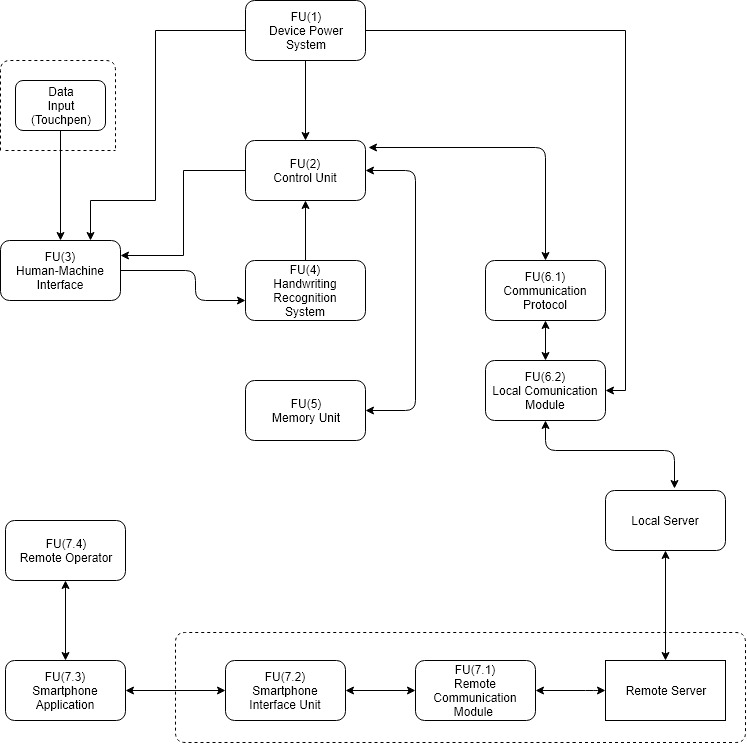
\includegraphics[scale=0.63]{blockchan.jpg}
	\caption{Functional Block diagram of the system to be developed.}
\end{figure}
\clearpage
\noindent
FU1, the device power system supplies power to the embedded control unit, FU2, which controls the whole system on the device. It also powers the modules that are responsible for the wireless transmission of the user's shopping list to their smart-phone, FU6.2. \\
All processes that happen on the device go through FU2. It is the root of the device, in other words if it breaks down, the whole system will not work and if it is faulty, the whole system will be faulty. Therefore, debugging mainly starts from FU2, to the other sub-components dependent on it.\\
FU3, the human-machine interface, is responsible for inputting the user's shopping list to the control unit in their own handwriting. It also displays the output received from the control unit. There is direct interaction with the user acting as the local operator.\\
Handwriting input from the user is converted to readable text, via FU4, the handwriting recognition system. A timer system is implemented within the system so that after a specific amount of time, data on FU3 is passed to FU4, which scans the data and compares it to a initially trained data set within FU4 and outputs the string that is learned from the data set. The recognition and learning process is implemented by use of back-propagating neural networks.\\
The inputs from FU3 will be words that will be on a line on FU3. A word segmentation algorithm is used to split each word into characters by use of the spaces between the handwritten characters that make up each handwritten word. The segmentation algorithm also contains a way to recognize space between full words that are input by the touch-pen onto FU3. This space is larger than the space between characters. Each raw input letter that is obtained after segmentation is then converted to the nearest learned text letter using the handwriting recognition algorithm. The converted letters are then concatenated after conversion of every letter on the line, to form the full words contained in the input line, in text. In the process of full-word integration, comparisons are made between succeeding characters to determine if they make grammatical sense next to each other. If not, the user is given the option to enter these words again, and if the learned words are the same, a suggestion for possible intended characters is displayed, with the user being given the option to keep the characters they entered or correct their input with the suggestions. The line containing the converted words with spaces between them, in text format, is displayed on the upper part of FU3 and the user inputs the next line onto the bottom part of FU3 that prompts for the user's next shopping item data input. The input line of handwritten text is converted to text using the previously defined method and the output is appended to the line after the previously converted line. This process continues until the user enters their full shopping list. \\
After FU4 successfully converts the user's shopping list input, the training data is updated with the input data that will just have been successfully converted. The training data is updated in a First-In First-Out manner with the assumption that the training data just obtained will most likely look like the data input to be input in the near future.  
FU4 passes the converted text to FU2, the control unit so that the text is saved to the memory of the system, FU5. \\
Information is sent to the user's smart-phone through FU6.1, the communication protocol. The user's phone has an in-built communication system, FU7.2 which interacts with FU6.1, the local communication module of the device. The shopping list input by the local operator is obtained on the smart-phone via FU7.3, the smart-phone application. The user requests the shopping list via the remote operator, FU7.4 which controls FU7.3.
\clearpage
\newpage

%% End of File.



\section{Target Specifications}

\subsection{Mission-critical system specifications}
\begin{center}
	\begin{longtable}{|p{5cm}|p{5cm}|p{5cm}|}
		\hline
		\textbf{SPECIFICATION} &
		\textbf{ORIGIN} &
		\textbf{VERIFICATION}\\
		\hline
		Information should be sent at request, to the mobile phone within 10 seconds.
		&
		The customer needs the shopping list sent to them as quickly as possible, but accounting for internet downtime, firewalls and wireless signal strength, there are going to be delays in the transmission path.
		&
		A timer will be programmed within the mobile application to track the time taken between a  request for the shopping list and when it is received.
		\\
		\hline
		Accuracy of the handwriting character detection must be greater than 80$\%$.
		&
		A trade-off has to be made between conversion time and performance or accuracy. Additionally, with optimizing conversion time comes the downside of more cost since the processor memory for the conversions has to be increased.
		&
		Error rate calculation will be displayed every time a word is updated. \\
		% \hline
		% The device should send and receive information to a smartphone $\geq$5m away
		%    &
		% The device should interface with the smart-phone in a wireless manner %and thproves the two devices can communicate if one of them is anywhere in the city, provided there is consistent network access.
		%    &
		% Send a random text file from the device to the cellphone.
		%    \\
		\hline
		The system should recognize that the user has completed writing their shopping list.
		&
		Character recognition should start as soon as the user finishes writing their line in their handwriting to prevent the user from waiting for too long. Therefore if it is known that writing is complete, the recognition process can easily be triggered by a boolean flag.
		&
		A flashing white LED will be switched on 1 second after data input is finished.
		\\
		\hline
		The user must be warned when the battery power remaining is less than $10\%$ of full capacity.
		&
		The device has be on so that the list can be sent to the user's phone when they request for it.
		& 
		A red LED will flash on the device when the battery power is less than $10\%$.\\
		\hline
		Handwritten input must be converted to text by the character recognition software in less than 1s.
		&
		The user has to see if the converted text has errors and correct them as soon as possible before proceeding too far ahead with their text input process.
		& 
		An LED will be configured to switch on as long as conversion is not complete.\\
		\hline
		Text recognition should consider the probability of occurance of combinations of letters.
		&
		This reduces grammatical errors in the shopping list and reduces the search pool for the conversion of the next letter, reducing search time for the goal node containing the equivalent letter in the neural network.
		& 
		The device's touchscreen should display suggestions for consecutive characters that are converted to text but do not make grammatical sense next to each other.\\
		\hline
		The communication link between the device's communication system and the phone system should transfer data bidirectionally, at a rate of between $5 \textrm{Mbps}$ and  $10 \textrm{Mbps}$ so that the bit error rate can be less than 10$\%$. 
		& 
		The device should send the shopping list to the user's smart-phone at any mall in the city. A balance has to be found in the transmission rate because if the rate is too fast, the rate at which errors are generated during transmission increases, meaning the transmitted shopping list data will not be reliable with some letters being missed during transmission. However, if the speed is too low, then the user will be left waiting too long in the store for their shopping list to be delivered to them before they start doing their shopping.
		&
		Using linear programming methods to calculate the data transmission rate and display it on the touchscreen of the shopping list device \cite{Shannon:A_Mathematical_Theory_of_Communications}.\\
		\hline
		\caption{Mission-critical system specification}
	\end{longtable}
\end{center}
\newpage
\subsection{Field conditions}
\begin{center}
	\begin{longtable}{|p{7.5cm}|p{7.5cm}|}
		\hline
		\textbf{REQUIREMENT} &
		\textbf{SPECIFICATION} \\
		\hline
		The device should read handwriting input from multiple users. 
		&
		There will be more than 2 training sets for the handwriting recognition neural network that will be useful for conversion of handwritten data to text.   
		\\
		\hline
		The device should operate under varying light conditions that will be typical of what the user will encounter in indoor environments.
		&
		The device operates in a light intensity in the range of 50 lux  to 1000 lux.
		\\
		\hline
		
		\caption{Field conditions}
	\end{longtable}
\end{center}
\newpage
%% End of File.
%%
%%  Department of Electrical, Electronic and Computer Engineering.
%%  EPR400/2 Project Proposal - Section 5.
%%  Copyright (C) 2011-2018 University of Pretoria.
%%

\section{Deliverables}

\subsection{Technical deliverables}

\begin{center}
	\begin{longtable}{|p{7cm}|p{3.5cm}|p{3.5cm}|}
		\hline
		\textbf{DELIVERABLE} & \textbf{DESIGNED AND IMPLEMENTED BY STUDENT} &
		\textbf{OFF-THE-SHELF} \\
		\hline
		Optical character recognition algorithm for handwritten input to text conversion. The algorithm will be implemented on the hand-held shopping list device.  It contains the segmentation code for separating the handwriting input as well as the exception code for consecutive characters that should not be next to each other.&     X&  \\
		\hline
		Touchscreen for the user to write their handwriting input of their shopping list onto the shopping list device. It will also display the converted text from the optical character recognition software. The touchscreen will be part of the hand-held shopping list device.       &     & X \\
		\hline
		Mobile application on the user's cellphone to get the shopping list, saved on the shopping list device at home, sent onto the cellphone.         &   X  &  \\
		\hline
		Touch-pen used by the user to enter their handwritten shopping list items on the shopping list device's touchscreen. & & X\\
		\hline
		GSM module for the shopping list device's communication system so that commands can be received and information can be sent to the user's phone.& & X\\
		\hline
		Embedded processor board for the shopping list device's control unit.  & & X\\
		\hline
		Integration of the embedded processor board, the GSM modules and the LCD touchscreen to make the shopping list hardware device.  & X& \\
		\hline
		Assembly/C-Code to connect the Wi-Fi modules to the embedded system's serial ports and set-up a wireless connection.& X& \\
		\hline
		\caption{Deliverables}
	\end{longtable}
\end{center}

\subsection{Demonstration at the examination}
1. The demonstration will commence with the user pressing the device's power button. An option will be available for the user to write their list.\\
2. The demonstrator will then write a number of sentences on the touchscreen of the device and wait for them to be converted to text.\\
%2. The demonstrator will then write on the touchscreen of the device, a number of sentences and wait for them to be converted to text.\\
3. The demonstrator will then start up the Android application on the mobile phone. \\
4. The demonstrator will then press the button on the Android application interface, that requests the shopping list from the device.\\
5. The application will then display on the screen of the smartphone, the list of sentences that was put in by the demonstrator onto the touchscreen of the device in stage 2 of the demonstration.\\
\newpage

\bibliographystyle{IEEEtran}
\appto{\bibsetup}{\raggedright}
\bibliography{proposal}


%\putbib[proposal]
%\end{bibunit}
%}

% Reset the section counter
\setcounter{section}{0}

\newpage

%% End of File.



%% --- PART 4 ------------------------------------------------------------

\eprsec{Part 4. Main Report}
\newpage

%% Reset the page number style and count.
\pagenumbering{arabic}
\setcounter{page}{1}

%% Import the main report content
%%
%%  Department of Electrical, Electronic and Computer Engineering.
%%  EPR400/2 Final Report - Section 1.
%%  Copyright (C) 2011-2018 University of Pretoria.
%%

\section{Literature Study}

Two core designs are to be integrated for the successful development of the home shopping list device. These designs are the design for handwriting processing and device to device communication. The research done on the theory associated with these designs is discussed in this section.

Handwriting processing can be subdivided into handwriting recognition which is applied from the pre-processing to the processing stages and handwriting analysis, which is mainly applied in the post-processing stage. For handwriting recognition, the goal is to convert grey scale images of handwritten text into machine-recognizable code at an acceptable level accuracy. The user will write their shopping list data on the device’s touchscreen and the device must convert this handwritten data into ASCII text. The device’s handwriting recognition scheme can either be offline or online handwriting recognition. The different models from either of these schemes can be classified as either bottom-up or top-down models.

Bottom-up models involve the analysis of neuro-centric processes at the lowest level of abstraction. The processes analysed are those involved in the simplest input of a character to the full input of a handwritten word. Top-down models are most applicable to this project because they are familiar with language processing tasks like speech recognition. The models that are categorized as top-down can be sub-divided into discrete and oscillatory models. 

In discrete models, handwritten pen inputs are defined as the vector sum of the discontinuous pen strokes. On the other hand, oscillatory models classify oscillations as simple pen movements on the input surface therefore handwritten inputs are defined as suddenly interrupted pen movements.

In online handwriting recognition, a user inputs their data using a touch pen or any other stylus that provides a distinct pattern on the input surface e.g. ink. The stylus’s successive trajectories are recorded as vectors with x and y co-ordinates. This means the user’s order of inputting their characters is recorded in a 2-dimensional array. The recognition algorithm is then applied to these vectors and the input data is converted to ASCII text on the go. Therefore, the user gets real time feedback from the recognition scheme [2]. No recognition scheme can work perfectly so the advantage of this scheme is that incorrect conversions or errors can be corrected almost instantly. A timer is used so that after a certain period, when the pen is lifted or there is no input the array is saved. The recognition algorithm is applied to this array and the next time the stylus inputs another handwritten character, the saved already saved character has already been converted to the equivalent ASCII text and the array cleared. The next handwritten character’s co-ordinates are pushed into this empty array. If recognition is not finished, then another array is used. The arrays for saving the handwriting input therefore follow a queue format [6]. Queuing models are represented by Kendall’s notation. The typical Kendall’s notation is shown in the equation below.

\begin{equation}
	\text{Queue} = A/S/k
\end{equation}

In the equation, A represents the arrival rate. In the online handwriting recognition case, this is the rate that the vector arrays are saved. Since the time that a user finishes their input cannot be predicted and varies for each input sequence, it can be assumed to be non-deterministic and the cumulative time that the co-ordinates are saved can be assumed to follow an exponential series which can be modelled by a Poisson distribution. S represents the service rate. In the online case, this is the rate at which the saved arrays are converted to their equivalent ASCII text. This is non-deterministic as well and can be assumed to follow an exponential rate. This is due to the fact that the recognition rate has direct dependence on the sequence of co-ordinates in the array and these are non-deterministic. k represents the number of servers in the queuing system.  In this case the servers are modelled by the character recognition algorithm converting the 2-dimensional array into the equivalent ASCII code and clearing the array thereby freeing memory. This algorithm only operates on a single 2-dimensional array of the co-ordinates at a paticular time. No handwriting conversions can occur concurrently therefore the number of servers in the queuing system is equal to 1. The queuing system involved in the waiting for the array to be cleared can therefore represented by the model below:\\
\begin{equation}
	\text{Queuing model} = M/M/1
\end{equation}

Where:

\hspace{10mm} M = Markovian distribution which represents the arrival rate.

\hspace{10mm} M = Markovian distribution which represents the service rate.

\hspace{10mm} 1 = Number of servers.

Using the queuing model properties from [3], the average number of arrays used in the handwriting recognition process can be calculated. This leads to an easier calculation of the average amount of memory used in the online handwriting recognition process. This is calculated to be in the “Byte-range” in the worst case. This means this process is extremely memory-efficient since even the simplest everyday devices with micro-chips have millions of Bytes in memory at worst.

Online handwriting recognition is mainly focussed on three domains; digital signatures, pen-input devices and developmental tools. Digital signatures domain involves the use of well-trained recognition algorithms to verify a user’s identity to access important features e.g. bank account transactions. Pen-based device domain involves pen-input computer platforms recognizing handwriting or gestures from a user through a pen. Developmental tool domain involves the use of integrations of systems that take advantage of the neuro-centric property of handwriting recognition to develop and implement education and disability-assisting systems e.g. speech recognition algorithms to recognize and change voice to text for easier communication with the hearing-impaired. Our end goal is to develop a device that accepts touchscreen inputs and converts that to text. Therefore, this will fall in the pen-based devices domain. The domain is expanded to process electronic ink in the form of the pen’s drawing on the touchscreen.

Before the execution of the recognition phase, the handwritten input goes through a pre-processing phase. In this phase, noise is filtered from the input. Next, the skew within the pen input is corrected or normalized. The final stage of this phase involves the segmentation of the pen input into separate meaningful characters. Some models like Markovian models skip over this part to recognize the whole word that is input by the pen using probabilistic means which do not require segmentation. Therefore, segmentation is involved for models in which machine learning is involved.
There are various sources of noise for the handwriting input. The most common source is the user’s finger or hand randomly making contact with the touchscreen when the user intends to write using the pen. The capacitive touchscreen has no way of differentiating the pen from the fingers, so those motions are recorded as handwriting input. Another source of noise could be the pen used. Most of the pens used for touchscreens contain rubbers at their tips. The material used for the rubber directly affects the handwriting input. If the material is too large, then noise is introduced to the input by appending unwanted features to the drawn characters or words. However, the tip has to be large enough for the drawn input to be recognizable, so a trade-off is made for the right type of pen to have a significant size for its tip as long as the noise it produces is filterable or small enough to be differentiable from the actual input. Another source of noise is the touchscreen’s drawing application introducing a certain amount of quantization noise. Noise can be removed from the handwriting input by digital processing methods like signal filtering and data smoothing [5].

Skew normalization is normally applied to recognition systems which accept cursive word input. In this case, the slant on the skewed word is checked against a certain limit that is pre-defined e.g. a maximum of 45o to the right. Therefore, the required skew adjustment angle will be calculated by finding the difference between the skew angle and limit e.g. 45o in this example case. If the skew angle is less than the limit, then no skew correction is necessary.
\begin{equation}
	skew_{correction} = skew - limit
\end{equation}

The skew above the limit is compensated for by shifting the cursive by the value of $skew_{correction}$. 

Segmentation applies at two levels. In the first, it is involved in the separation of equations, lines contained in a paragraph into different lines and the words in a specific line into different words. At this level, spatial zones [6] are defined so that trivial units are extracted from a paragraph. This level works for inputs which are provided in a paragraph format. It could also work in the practical case for line inputs by separating the line into different words of shopping list items. In the 2nd level associated with segmentation, input is separated into individual characters. This is lowest level of segmentation of importance. Therefore, after the paragraphs are segmented into separate lines and lines are segmented into different words, the different words contained in each line are separated into individual characters. This is hardest part of the pre-processing phase because it involves the separation of cursive words into individual characters. Separating cursive words means determining where each character starts and ends. The obvious risk is that a character’s features can be incomplete and be appended to the next character’s features leading to a character that is incomplete and another that is unknown. This error carries over to the recognition process where the probability of recognizing both these characters correctly is reduced. Most segmentation is carried immediately before the recognition process by using machine learning, namely convolution neural networks to separate the cursive text into characters.

The recognition process can be split into two classes, rule-based methods and structural methods. Structural methods involve the abstract definition of character shapes [7]. The shape variations involved in the practical real-world applications of the recognition process are ignored. Rule-based methods involve the use of flexible rules that use statistical models to determine frequency of occurrence of certain features [8] in a shape. The statistical models associated with these methods can either be explicit, implicit or Markovian. Explicit statistical models generally follow linear distributions, but they require a lot of memory and processing speed. Implicit models involve the use of natural networks for the training of pen input and learning from predefined test results. Error correction is done by using by using back-propagation in the neural network and the future handwriting input learns from the already tested dataset. Markovian models involve an under-the-surface process whereby state changes occur depending on the conditional probabilities associated with each state. Markovian models can be used as a work-around segmentation when dealing with cursive word input.

On the other hand, when offline handwriting recognition is used, the whole document is scanned. This scanned document is converted to an image and the recognition algorithm is applied to the whole image so that the whole paragraph is converted to the equivalent ASCII text. An interrupt can be programmed so that scanning is done periodically. The user only gets feedback from the scheme after the whole document has been scanned and converted to text.

The same pre-processing steps applied in online handwriting are usually applied to offline handwriting. The image taken from the scanner must be converted from grey-scale to binary in the step called thresholding. In the binary converted image, the scanned input will now be in black and white. The binary values of 1 and 0 are assigned to the two colours. The image is different into any pixels and each pixel is represent by a bit. A bound is pre-set to define the border between a pixel which is black and one which is white. The bits representing the pixels are then added to a 2-dimensional array. The rows of the array contain the pixels of the image in the width spectrum while the columns represent the image pixels in the height spectrum. It is important to note that this array is the one that is the argument of the recognition algorithm after the segmentation and other noise removal processes. 

Since digital capture is the most popular image capturing technique in offline recognition, noise is inherently most likely to occur from the device used to scan the images. These disturbances can be rectified using a smoothing process. Another popular problem associated with offline recognition is the overlap of successive lines in a paragraph due to skewing. A possible solution is the use of thinned images to follow the scanned strokes linearly and segment the interfering strokes from the signal. Instead of removing this signal, it’s coordinates, and shape are noted and appended to the next thinned line which will be missing this information. This correction may require skew correction on the part of the segmented strokes. 

For many skewed scanned images, the approximate skew angle is similar globally. An example is shown in the image that follows.\\
\newpage
\begin{figure}[h]
	\centering
	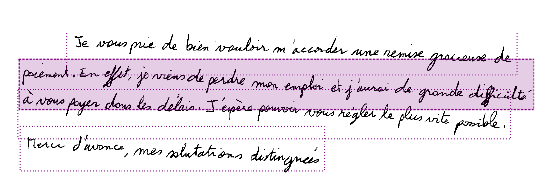
\includegraphics[scale=0.9]{1}
	\caption{An example showing global skew in a scanned image}
\end{figure}
\nocite{Haykin:Communication_Systems}
The scanned handwritten paragraphs have to be segmented into lines, then into words and finally into characters. The task of line segmentation is complex since handwritten text is normally written into non-symmetrical imaginary lines and these lines overlap up and down as shown in Figure 2, thus affecting neighbouring lines’ line input. The most popular method is estimating global angles of both vertical and horizontal skew. These angles are normalized as is done in online recognition skew correction. The space is repeated from the assumed initial line of the image to the last line. The local minimum of each captured line is approximated to be the baseline [104] for each line and these minima are concatenated to classify all the lines. For word segmentation, each segmented line is then split into its constituent words. The most popular scheme is using a rule-based approach where physical gaps are defined and if the gap size or higher is encountered, then a preceding word is separated from the next one. The assumption in using this approach is that the space between consecutive words is assumed to be bigger than the space between consecutive characters in a word. After separating the line into words these words have to be converted to ASCII text. These words are either passed to the recognition algorithm or they are further segmented into different characters. Word-level recognition uses statistical models which are discussed later. Most of the recognition schemes require character input so the words need to be further split into characters. Special features like concavities [102] are incorporated to determine segmentation points. The segmentation algorithm incorporates rules that compare gaps between segments to obtain the different characters.

A major difference between the pre-processing steps of offline and online handwriting recognition is that character segmentation in offline recognition is normally associated with non-cursive text while online recognition normally deals with cursive handwriting input.

The word-recognition algorithm is used, and the word image is compared to options in a lexicon and a list of the most probable words is returned. The recognition approach can either be holistic or analytic. When a holistic approach is used, the whole word image is immediately converted to equivalent ASCII text normally by statistically based models. On the other hand, an analytical approach recognizes the segmented characters of the word and then combines the results at the end.

Comparison between the two handwriting schemes shows that it is easier to correct conversion mistakes when using online handwriting recognition since feedback is provided after each character input. In contrast, since a whole document is scanned in offline recognition there will be multiple mistakes observed after each conversion and correcting these errors is a lot of work compared to when using online handwriting recognition. This is because conversion in offline recognition is on a paragraph level, which means in the worst case, there will most likely be errors for every word, in every line in every paragraph. In comparison, the worst case in online handwriting is an error in recognizing the preceding character which is far easier to fix by just rewriting the character.

Most handwriting recognition schemes have their accuracy dependent on how close the user’s handwriting is to the standard training sets, which are the IAM and the MNIST data set. The home shopping list device to be developed adds onto the already used datasets so that multiple user handwriting styles can be converted to ASCII text at an acceptable accuracy level, which is 80$\%$ or more in this case as shown in the project proposal section.

A hybrid of the two recognition schemes will be used in this project. Shopping list data will be input onto the touchscreen line by line. A touch pen will be used to input each line, as is done in online recognition and after each line the user will click a button to convert the line. After this button is clicked, the user input on the touchscreen will be converted to an image, as is done in offline handwriting recognition. The recognition algorithm will then be applied to convert this image into a line of text. This method makes use of the best traits of both online and offline handwriting recognition. Recognition is done on a word level, meaning a dictionary can be used to disregard character recognition errors. This dictionary contains a list of pre-defined words, in this case words that are normally found in a large-scale grocery store. 

The methods that have been developed to solve this problem are statistical models like Hidden Markov Models and machine learning models like neural networks. Hidden Markov models involve the use of probability distributions to calculate the chances of state transitions which relate to the probabilities of certain words being next to each other for character recognition. An algorithm called the Viterbi algorithm is then used to connect and detect the most likely sequence detected, which is not necessarily the most likely characters detected but the most likely word handwritten. On the other hand, neural networks work mostly with individual character recognition, with the emphasis being on training the network enough so that it can correctly detect unseen handwritten data passed to it. It is clear that the best scheme is somewhere in the middle of the two schemes analyzed so the best way could be integrating them and taking the best features provided by each scheme. 

The device to device communication design is useful for communication between the shopping list device and the user’s mobile phone. The various communication techniques available are grouped into either wireless or wired communication. The user will need to send a text-file containing their shopping list from the shopping list device to their mobile phone.  

Wired communication involves the direct use of cables and wiring for the transfer of data. The most popular application of wired communication is the use of a telephone. The telephone is connected directly to the local telephone switch using wires from the user’s home to the local telephone switch station [48]. The wires used could either be copper wires or optical fibres. Most modern wired systems use optical fibres because they are capable of carrying more signals compared to the traditional copper wires. Telephone service providers usually provide internet access with the same wiring using used for basic telephone communication. A splitter can be used to allow a single incoming wired connection to provide both internet access as well as the basic audio network for making and receiving calls. Wired connections are the most stable and are not easily affected by weather. When a wired connection is used instead of a wireless communication the signal strength will be higher and the transmission speed will be faster. 

The most popular type of wire used is the twisted pair wire. This type of copper wire is used for both the transmission of data as well as basic telephone communication. This wire achieves one of the fastest data transmission rates possible i.e. 100 Mbps. Although the wire is cheap, it can only cover a maximum distance of 100 m which is way below the desired transmission distance which is limitless. Another type of wire used in wired communication is a coaxial cable. The cable contains a copper wire at the centre surrounded by insulation tape. Transmission speeds can reach up to 10 Mbps and it is mainly used in television broadcast transmission as well as broadband communication. The fastest growing cable used in wired connections is the fibre optic cable. The most important property of these cables is that each cable contains thin plastic strings that carry data by reflecting light. The strings can be made of glass to increase the cable’s reflecting capability. These cables can transfer data at speeds of up to and greater than 10 Gbps.

The use of wires in this communication scheme means that the connections are susceptible to corruption by physical means [49]. Some of these data corruption mechanisms include attenuation. Data transmission can also be delayed due to earthquakes or other natural disasters that may affect the wires for the connection. Since copper wires have to be used for long distances where homes can be up to 30 km from the central station, they cannot be under surveillance for all this distance in remote areas and are thus susceptible to theft. Wired communication is most adequate for real-time high-bandwidth requiring operations like live video streaming.

On the other hand, wireless communication techniques do not use wires in data transmission. Wireless communication techniques are designed to cater for hinderances, mainly physical, associated with wired connections therefore they are more convenient than their wired alternative. These are the most popular communication techniques and are categorized depending on the range they cover. Infrared transmission is a technique where data is carried from one device to another using waves near the infrared spectrum as the transmission medium. Infrared communication is extremely range-limited.  The range covered by an Infrared connection can be extended by using high-powered infrared lasers which can be dependent on broadcast or point-to-point. For point to point infrared transmission the devices on which the technique is implemented on should be physically visible to each other with no obstructions between them. In contrast, broadcast transmission transmits the data in all directions, so the devices need not be facing each other but there should be no obstruction between them. Broadcast transmission introduces security threats as any device in range of the connection can pick up the data broadcast by the sender not intended to be for every device. Modern examples of Infrared applications are television remote control systems. 

An alternative technique to infrared transmission is radio transmission. In this technique, radio frequency for communication ranges from 30 Hz for basic submarine applications to 30 GHz for wireless LANs. Frequencies in the 100 GHz range are used for microwave communication. The signals in the radio spectrum should propagate between the cell site antenna and the device’s wireless terminal. Therefore, for successful communication, data is sent from the sender and it is picked up by the receiver’s antenna. Radio transmission penetrates obstacles like walls and oceans/seas.

Bluetooth is an example of a radio transmission technique. In this technique, digital data is transmitted wirelessly between connected devices within a range of up to 30 m away from each other. The communicating devices can be separated by a wall and data can be successfully transmitted as long as the distance between them is less than 30 m. Similar to Infrared transmission, the transmission speeds of Bluetooth only peak at 1 Mbps. Bluetooth and other radio transmission schemes involve the use of encryption algorithms and authentication schemes which make sure that even if data transmission is broadcast only the intended receiver will be able to access it by using a pre-defined security key and the receiver will be able to know and verify the correct sender. Another example is WLAN transmission. WLAN transmission range is significantly larger than the one used for Bluetooth. It typically extends to a few hundred meters. WLAN, typically known as Wi-Fi also transmits data about 10 times faster than Bluetooth with its transmission speeds being as large as 11 Mbps. WLAN is not completely cable free since it needs the router to be connected to the main network via a cable. The end-user devices are the ones that have a wireless connection with the router and thus with each other.  The shopping list device can communicate with the user’s phone by using a WLAN to connect to the Internet. The Internet is used as a workaround to bypass the transmission distance limitation. This means the two communicate via the Internet with no need for them to be in the same geographic area. WLAN also has a built-in firewall therefore enhancing the security of data transmitted by devices using this network.

There are different types of wireless networks available for analysis before choosing and implementing the correct communicating module. The most popular network is Local Area Network. In this type of network, the communication is between device and the user’s phone, but they are restricted to be in the same geographic area. This limit is detrimental to cases where the user travels even a few miles to work and intends to do their hopping on their way back home. An alternative is explored, and it is found in the form of Wide Area Network. This network covers a wide geographic area, typically cities or entire countries in some cases compared to LAN which is restricted to a maximum of 100 m [9], so WAN is more desirable for the device’s communication system.

The communication system of the device to be developed will be a WAN and can be implemented using either GSM or LTE. An advantage of GSM is that it works well for both data transmission and voice at a relatively low price. In comparison, LTE works well for data transmission but costs significantly more than GSM to implement. GSM modules are also adaptable and user-programmable for various devices while LTE instead works best on cell phones. The shopping list device is not a cell phone thus integration with LTE if chosen as an option, would suffer from the previously described drawback.

The wireless techniques used for communication can be grouped into 2 groups. They can either be packet-based techniques or circuit-based techniques. The analogues signal if first converted to digital form for both techniques. Packet-based wireless systems group the bits to be transmitted and transmit them in packets, only when a transmission request is made [6]. In circuit-based systems, when a connection is made, a reservation is made so that no other user can use this connection while still connected. This makes circuit-based systems ideal for real time communication, which is not of interest to this project [7]. Packet-based wireless communication associates most closely with the desired communication scheme of the device to be developed. This is because communication will only be done on request unlike circuit-based communication which results in high data costs due to the receiver always being in acquisition mode because of the continuous communication property of this type of communication.

The Internet of Things is the connection that will be set up between the shopping list device while attached on the fridge at home and the customer via their phone. The information on the shopping list device will be global and the user’s phone will be interconnected with it.

A wired connection is not ideal for this project because the device will need to be attached to a fridge and there should be no bound on the transmission distance i.e. the user should get the shopping list sent to them when they request it wherever they are. The proposed connection will be a wireless connection which will communicate with the user’s cell phone. 

\newpage

%% End of File.



%%
%%  Department of Electrical, Electronic and Computer Engineering.
%%  EPR400/2 Final Report - Section 2.
%%  Copyright (C) 2011-2018 University of Pretoria.
%%



\section{Approach}

The design for the system, as explained in the previous section should contain two main designs, handwriting recognition and communication.

\subsection{Design alternatives}

The data input device to be used to input data onto the device’s touchscreen could either be a light pen or a mouse. The trade-off associated with the choice for the device was that of portability against the degree of detail of the drawing painted on the touchscreen interface by the input device. Another trade-off considered was that of pressure sensitivities on the touchscreen which would gradually damage the touch screen’s display against the degree of detail that would be provided by the input device. 

The Human-Machine Interface functional block could be designed for by comparing the different touchscreen devices available. The available choices were capacitive touchscreens and resistive touchscreens. A trade-off for the touchscreen device to be chosen was that of sensing pen or data input gestures using the chosen data input technique but filtering out input that was not from the data input device like a user’s palm interfering with the drawing while the user was holding the device. 

The device’s control unit block could be designed for using either a micro-controller or a development board. A micro-controller had an advantage of being small. A development board had an advantage of minimizing the overall device’s wiring. If a micro-controller were to be used, a PCB would be required to integrate it with the touchscreen and the communication module to be used. The micro-controller would also need to be integrated with an external microprocessor as well as an external memory module for saving the shopping list data and I/O pins for external serial interface. This would result in a lot of wires in the system that would affect debugging time if mistakes were made. On the other hand, development boards have the microcontroller, the microprocessor, sometimes communication modules, a memory module slot and just about enough I/O pins all on the same lightweight board. Development boards are also programmable using high level programming languages like C++ and Python, making them easier to simulate on PCs.

The handwriting system process is shown in the diagram on the next page.\\\\
The Recognition Algorithm could be designed and implemented using Neural Networks or Hidden Markov Models. An advantage of the neural networks approach was that with increased training data, unseen patterns of line handwriting inputs could be accurately recognized. An advantage of Hidden Markov Models was that the probability of characters being next to each other is considered to estimate patterns with predefined data sets, producing words which are in the dictionary.
\newpage
\begin{figure}[h]
	\centering
	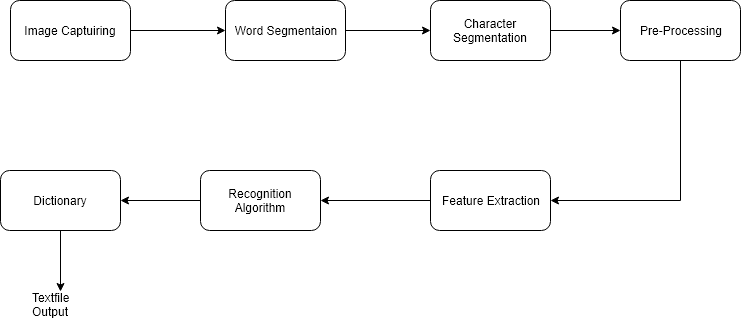
\includegraphics[scale=0.5]{2}
	\caption{Basic Flow diagram showing the modules associated with the handwriting recognition process}
\end{figure}
A diagram of how the general communication is achieved for the device is shown below.
\begin{figure}[h]
	\centering
	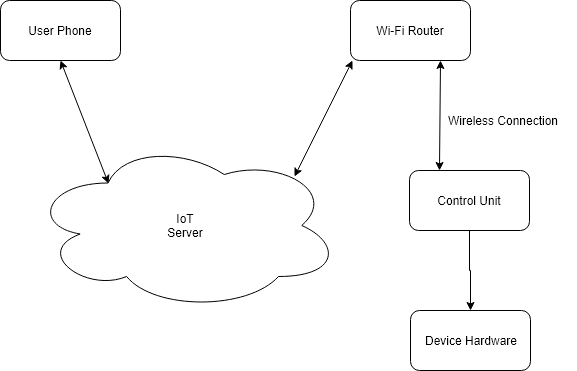
\includegraphics[scale=0.5]{3}
	\caption{General communication system for the device}
\end{figure}

The communication system of the device could be designed and implemented using either GSM communication or Wi-Fi communication. An advantage of GSM is that high speed data transmission is possible. Also, with enough money to cater for roaming costs, data could be transmitted between two devices situated anywhere in the world. An advantage of Wi-Fi is that the network is secure is broadcast data signals can be transmitted to the other device if they have the correct pre-shared key. 

The mobile application to access the shopping list can either be the phone’s SMS system, the phone’s email system or a customized application. An advantage of the SMS system as well as the e-mail system is that it prints the text as it is from the text document from the shopping list device and the. An advantage of the customized application is that it presents the shopping in a more customer-focussed user interface. A button only has to be pressed and the user can access their list.

\subsection{Preferred solution}

A touch pen (stylus) was chosen as the design choice for the input device to be used. This was because a pen more accurately defined a real-world handwriting drawing since in the real-world people use pens and pencils to write. Additionally, a pen is portable and wireless while a Bluetooth connection first is needed for a wireless mouse and the shapes drawn by mice do not accurately model human handwriting styles. An important trade-off when eventually getting the off-the-shelf stylus pen was the pen size against the precision. Bigger stylus pens can be sensed more easily by a touchscreen device, but the drawings produced by them are not precise enough to model real-life handwriting. An optimum size of the pen was supposed to be chosen for portability purposes and reasonable tip size.

A capacitive touchscreen was used as the HMI of the system because it is less susceptible to scratches and permanent damage when a light pen is gently pressed onto the screen compared to resistive screens which require more rigorous pressing for pen drawing detection thus causing the screen to be easily damaged. The trade-off associated with the screen is that of the requirement that it should provide enough visible space for comfortable handwriting input while being small-scale enough to be integrable to the rest of the hardware and keeping the whole device lightweight.

A development board was used for the control unit of the shopping list device. It was chosen because it reduced wiring as explained before and it could easily be simulated on a PC. The development board of choice would have to run an Operating System that also runs on PCs. A trade-off associated with using a development board was finding the optimal price of the device which contained most of the hardware for the desired embedded circuit so that programming the hardware was the most complex part to be done on the control unit. The choices of development boards available to use for the device will vary from Raspberry Pi, to Odroid and Adafruit boards.

A neural network approach was used because the accuracy of the recognition process could be improved as more patterns were input into the system and the algorithm was trained and learned from previous results. A trade-off of the neural network approach was sacrificing accuracy for conversion time. An optimal number of hidden layers was calculated and used so that conversion time could be less than or equal to 1 second as specified in section 3 of the document while the accuracy could be 80% or more. The algorithm was programmed using the Python programming language.

Wi-Fi communication was used instead of GSM. This was because GSM has recurring costs associated with the service provider used and reloading the service requires removing the SIM card from the GSM module, recharging it on a cell-phone and inserting it back onto the module. The device to be developed will be permanently enclosed except for its charging system so this interferes with this condition. Alternatively, recharging is done by complex programming. On the contrary, reloading the Internet service for Wi-Fi is done on the router and no hardware on the shopping list device is interfered with. A trade-off associated with Wi-Fi communication is that of power consumption against transmission speed. [1]. Since the desire is to transmit data over a long range, an optimum speed should be designed for where the device does not run out of power whole in the process of transmitting the shopping list data.

The e-mail system application was used because this is an everyday application that most cell phone users are familiar with. A customized application was to be additionally programmed using Android Studio instead of Qt due to its mobile-focussed platform for mobile application development.

\newpage

%% End of File.


%%
%%  Department of Electrical, Electronic and Computer Engineering.
%%  EPR400/2 Final Report - Section 3.
%%  Copyright (C) 2011-2018 University of Pretoria.
%%

\section{Design and implementation}


\subsection{Theoretical analysis}

The project was divided into two interfaces that would be integrated after they were complete to produce the final device. These were the handwriting recognition process and the communication process.

The handwriting recognition process required the analysis and understanding of natural language processing and machine learning. Computers gain the ability to make decisions based on calculations done by the use of machine learning. Machine learning involves the use of neural networks and statistical approaches like Hidden Markov Models.

When neural networks are used, computers have the ability to learn through implementations of algorithms that make use of these neural networks. A neural network is modelled after the human brain which has billions of neurons. Each of these neurons is connected to thousands of other neurons and these neurons exercise extensive parallel processing, helping the human brain detect information and make decisions in a very short burst of time. In the case of handwriting, a person sees a handwriting and then detects the words written. This may seem like a short trivial process, but a lot of processes are involved in the process. A picture of the handwritten word is passed to the brain. The brain feeds the information from the image to its neurons. Before this image is obtained however, the human must have learned about the characters in the alphabet and many patterns that they come in. The brain is trained with previous data to detect the characters in the word. For unrecognizable characters, the brain uses common sense to detect the most likely character to form a full word that makes sense. 

Neural networks do not work the exact same way, but they make use of the most important part of the brain, learning. A neural network that works close to the human brain contains millions of artificial neurons inter-connected to each other. When the cumulative input to a single neuron exceeds a certain threshold value, the neuron changes from an off state to an on state. The activation output is transmitted to other neurons that depend on this neuron. Because of neural networks’ capability to learn, they can generalize data well. When trained well enough, a neural network can find solutions to unseen data that is not part of the training set. In the scope of the project, the neural network should therefore be able to generalize for unseen handwriting inputs that are not part of the training set. This unseen handwriting will be known as the test set and this test set will be compared with the expected text output to find the accuracy of the neural network implemented. An important consideration is that the unseen data input should be under conditions similar to the training data therefore it is important for the unseen data to be noise-free. 

To incorporate the parallel processing property of the human brain into the neural network, the 100-step rule is applied. The human brain typically recognizes familiar objects in approximately 100 ms. The neuron switching time is approximately 1 ms. The number of time steps of parallel processing associated with the brain are equal to:

\begin{align*}
	\text{Number of steps} &=  \frac{\text{Recognition time}}{\text{Switching time}}\\
	 &=  \frac{100\text{ ms}}{1\text{ ms}}\\
	 &= 100 \text{ steps}
\end{align*}

	This corresponds to 100 assembler steps and it is not feasible for a computer using the 100-step rule to do anything. Therefore, the limitation is that neural networks cannot work as well as the human brain but can be modelled after it.

To get an accurate foundation of how neural networks work, the human brain is first analysed. The part of the body that processes information is called the vertebrate nervous system [11]. This system has a central nervous system which consists of the brain and the spinal cord. The rest of the human body’s nerves are part of the peripheral nervous system. Since the neural network model resembles the brain the central nervous system was looked at more closely.

The central nervous system acts as the CPU of the human body. The CNS manages all the information in the body. The brain is the important component to be analysed for the model to be designed. Within the brain are billions of information processing cells called neurons [12]. The trivial definition of a neuron is that it is a switch with an input and output. Multiple neurons contribute to the input of each neuron and if the sum of these neuron inputs is greater than a certain threshold, the switch is activated. \\
\begin{figure}[h]
	\centering
	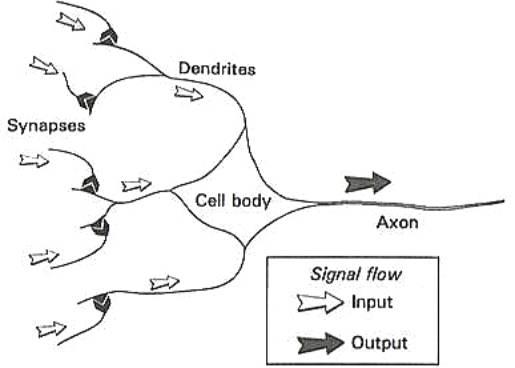
\includegraphics[scale=0.6]{4}
	\caption{Visual representation of a biological neuron}
\end{figure}

	Synapses receive the signals from the input neurons connected to that particular neuron. When a signal is received by the synapse, it is directly transmitted to the nucleus of the neuron. Dendrites receive the synapses that carry the signals from the input neurons and carry them to the nucleus of the neuron. The neuron’s nucleus sums up the inputs from the dendrites and when the summation exceeds a certain threshold value [13], an electrical pulse is activated. The neuron’s axon then transmits this pulse to the neurons whose inputs are connected to this neuron. Approximately 100 billion neurons are found in the human body.

The computer system executing the handwriting recognition process will model the biological neurons using artificial neurons. Artificial neurons are mathematical functions modelled after biological neurons to assist computers in learning like the human brain does. 

\begin{figure}[h]
	\centering
	
\includegraphics[scale=0.6]{5}
	\caption{Visual representation of an artificial neural network}
\end{figure}

An artificial neural network containing a single neuron layer is known as a perceptron. The perceptron takes vectoral input. This is information from neurons connecting to the input of the artificial neuron. In Figure 5, the inputs are the x values. These are typically contained in an array. They are represented as follows:
\begin{equation}
\text{Inputs}: \vec{x}= [x_1,x_2,x_3,x_4,..., ..., x_n]
\end{equation}

The vectorized inputs undergo a pre-processing phase where they are multiplied one-to-one with the vectoral weight components. The weights enable the perceptron to make conclusions from the inputs, giving each input a measure of significance. A significant part of the knowledge of the whole neural network therefore lies in the weights. The weights are represented as follows:
	
\begin{equation}
\text{Weights}: \vec{w} = [w_1j,w_2j,w_3j,w_4j,………,w_nj]
\end{equation}

The transfer function sums up the products of the inputs and their relevant significances to produce a single scalar value. This process is shown below:
\begin{align}
net_j &= x_1\cdot w_{1j}+ x_2\cdot w_{2j}+x_3\cdot w_{3j}+x_4\cdot w_{4j} \nonumber  \\
net_j &= \sum_{i=1}^j x_i \cdot w_{ij}
\end{align}

This value then undergoes a threshold test to determine if the neuron is switched on or off. This threshold test is known as an activation function. A trivial case of a simple threshold test is shown in the pseudo-code that follows.
		
\begin{algorithmic}
	\IF {$net_j > \phi$} 
	\STATE $\phi_j \leftarrow \textbf{ON}$
	\ELSE
	\STATE $\phi_j \leftarrow \textbf{ON}$
	\ENDIF 
\end{algorithmic}

In this case, if $net_j$ is greater than $\phi$ then the perceptron is activated by switching on its output while, if $net_j$ is less than $\phi$, the perceptron is not activated. The final output of the perceptron after the activation process is stored in $\phi_j$. The general activation function is represented by the symbol f and it calculates the exact value of $\phi_j$.

\begin{align}
\phi_j &= f(net_j) \nonumber\\
\phi_j &= f\big(\sum_{i=1}^j x_i \cdot w_{ij} \big)
\end{align}

An inter-connection of neurons is called an artificial neural network. A neural network is made up of neurons and weighted connections between them. The weighted connections transport output from the output of a neuron to the input of a dependent neuron. A simple example of a neural network is shown in the figure that follows.

\begin{figure}[h]
	\centering
	
\includegraphics[scale=0.6]{66}
	\caption{Visual representation of a basic neural network}
\end{figure}

For the simple neural network in Figure 6, initial inputs i1 and i2 are weighted differently as they are passed to the hidden layers neurons h1 and h2. The i1 input to h1 is not necessarily the same as the i1 input to h2. This is because the connection to each of h1 and h2 is unique and independent to each other so the product of the weight and the scalar value from i1 is the input value to h1 or h2:

\hspace{20mm}i1 input to h1: $w_{i1-h1}\cdot i1$

\hspace{20mm}i1 input to h2: $w_{i1-h2}\cdot i1$

From the expressions above $w_{i1-h2}$ and $w_{i1-h1}$ are unique and different. The basic steps associated with any neuron in a neural network are shown in the figure below.

For a simple neural network, each neuron can be modelled to process data in the format shown in the diagram below.

\begin{figure}[h]
	\centering
	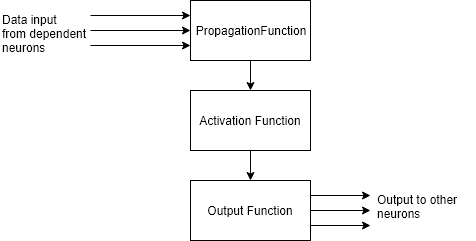
\includegraphics[scale=0.7]{7}
	\caption{Data processing functions in a neuron}
\end{figure}

The data input from each neuron is multiplied by the relevant weight to provide the input to the argument neuron. The propagation function is responsible for summing up the data inputs after different neurons after they have been multiplied by their relevant weights. These products are summed up to form a singular net input. The net input produced by the propagation function is passed to the activation function. The following mathematical functions describe the process associated with the propagation function.
	
Given a set of neurons, $I_s= \{i_1,i_2,i_3,…,…,i_n\}$ and the weight values for each neuron $w_{iz,j}$ are unique and independent ,and $z\, \varepsilon \, \{1,2,3,…,…,n\}$ , the cumulative network input to the neural network is calculated by the propagation function, $f_{prop}$ as follows:

\begin{align}
	net_j &= f_{prop} (\text{output}(I_s ),\text{weights to j}(w_{iz,j})) \nonumber \\  
net_j &=f_{prop} (o_{i_1},o_{i_2},o_{i_3} ,…,…,o_{i_n},w_{i1,j},w_{i2,j},w_{i3,j} )	
\end{align}

	
The input from each input neuron is the product of the weight to the argument neuron and the output from the input neuron. Therefore:

\begin{align}
	net_j = \sum_{i\, \varepsilon \, I} o_{i} \cdot w_{i,j}
\end{align}

The sum of these neuron inputs is shown in the equation above to be stored in $net_j$. This value of  $net_j$ is the value that is passed to the activation function in Figure 7. The activation function introduces non-linear properties to the network input. If an activation function were not to be used, the output would be a simple linear function whose polynomial degree is equal to 1. This type of polynomial has less ability to learn complex mappings. The activation is global for every neuron in the neural network and if the neural network has no activation function, it is known as a Linear Regression Model. A plot of this activation function is shown below:

\begin{figure}[h]
	\centering
	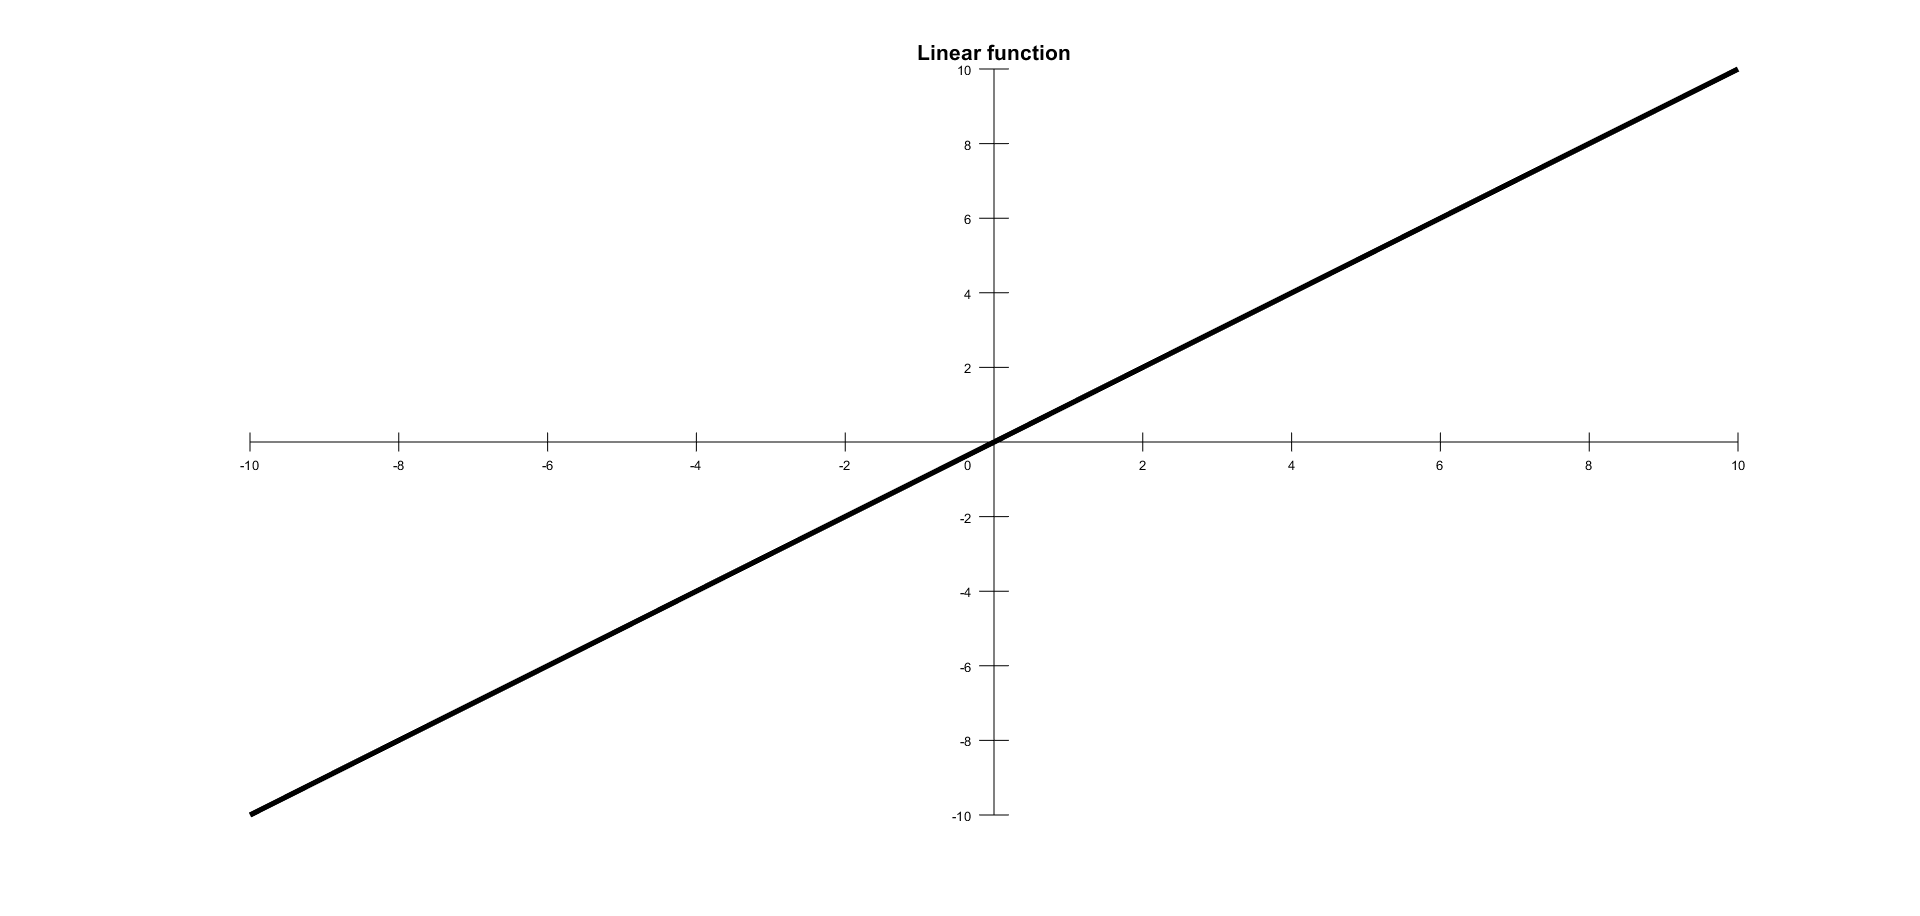
\includegraphics[scale=1]{8}
	\caption{Activation function for a Linear Regression Model}
\end{figure}

A neural network using a Linear Regression Model cannot properly model and learn from data inputs in the form of images, audio and videos. The output $a_j$ from this activation function, $f_{act}$ is given by:

\begin{align}
	a_j &= f_{act} (net_j) \nonumber \\
	a_j &= net_j
\end{align}

If instead a non-linear activation function is used, the result $a_j$ will be vastly different. The simplest non-linear activation function is the Heaviside function, which was defined in the introductory neuron example in the section. If the network input from passed from the propagation function is above a certain threshold, the activation function output changes from one value to another. If the value from the propagation function is less than the threshold value, the activation output remains the same. A plot of a binary threshold function is shown below.
\newpage
\begin{figure}[h]
	\centering
	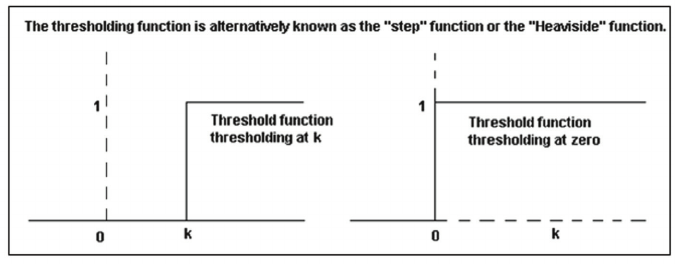
\includegraphics[scale=0.6]{9}
	\caption{Binary threshold function for k=0 and k$\neq$0}
\end{figure}

In this function, the x-axis values are the values from the propagation function, therefore the value of $a_j$ is calculated as follows:
\begin{gather*}
a_j :
\begin{cases}
	a_j = 1 & \text{for }net_j>k\\    
	a_j = 0 &  \text{for } net_j < k    
\end{cases}
\end{gather*}
It is important to note that the output values of $a_j$ do not necessarily have to be exactly 1 and 0 but they must be discrete and unique. As shown in the diagram, the values above and below the threshold are constant therefore their differential will be equal to zero since:
\begin{align}
		\frac{d}{d\,net_j} (a_j )&=\frac{d}{d\,net_j} (1)=  0 \quad \textbf{for} \quad net_j >k \\
		\frac{d}{d\,net_j} (a_j )&=\frac{d}{d\,net_j} (0)=  0 \quad \textbf{for} \quad net_j \leq k
\end{align}

The value of $a_j$ is undefined at $net_j=k$ and therefore is undifferentiable at this value. Due to this condition, it is impossible to implement the backpropagation learning scheme on a neural network using the Heaviside function as its activation function.

The discontinuity in the function also poses an important question. If all the initial input $x$ values are equal to 0 so that:
$$\vec{x} = [0,0,0,.....0]$$
Using equation (3.3):

\begin{align*}
	net_j &= \sum_{i=1}^n x_i \cdot w_i \\
	&= \sum_{i=1}^n (0) \cdot w_i\\
	&= 0 
\end{align*}

This result leads to a result $net_j = 0$. As shown in Figure 10, this result is at the transition point of the neuron being switched on for $k=0$. Most inputs are initiated to be vectors with zero values, so there is a risk situation that could arise. To avoid the situation where the net input is exactly equal to the threshold value of $k=0$, a bias input equal to 1 is appended to the inputs. This input will always be 1 and will also contain its own weight value. A representation of the new input system is shown below:

\begin{figure}[h]
	\centering
	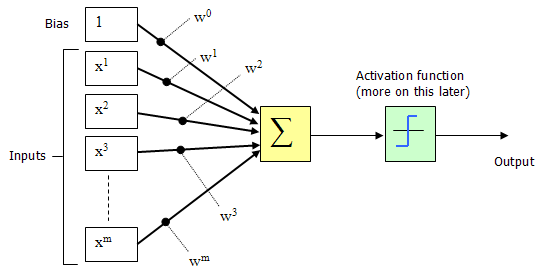
\includegraphics[scale=0.6]{29}
	\caption{Neural network with bias input}
\end{figure}

The above calculations apply primary to the Heaviside function with threshold $k=0$ which is the normally used activation function if a  Heaviside function is used. The equation to calculate the net input becomes:
\begin{equation}
	net_j = \big( \sum_{i=1}^m x_i \cdot w_i \big) + 1\cdot (w_o)
\end{equation}
When the inputs supplied are equal to a zero array therefore the value of $net_j$ can be calculated as follows:
\begin{align}
	net_j &= \big( \sum_{i=1}^m x_i \cdot w_i \big) + 1\cdot (w_o)\nonumber \\
	net_j &= \big( \sum_{i=1}^m (0) \cdot w_i \big) + 1\cdot (w_o)\nonumber\\
	net_j &= 1 \cdot (w_o) 
\end{align}

In the equation above, the weight $w_o$ will be the determining factor of $a_j$. If $w_o < 0 $, then $net_j <0$, therefore $a_j  = 0$ . If $w_o >0$, then $net_j > 0$, therefore $a_j = 0$. These conditions work for the Heaviside function with threshold $k=0$. The threshold $k\neq 0 $ is slightly complex for the inputs that lead to $net_j = k$ and adjusting them thus it is not commonly used. 

Alternatively, the logistical function can be used as the activation function. If this function is used, the activation output will be calculated as follows:
\begin{align}
a_j&=f_{prop} (net_j)\\
&=\frac{1}{1+e^{-net_j}}	
\end{align}

This function leads to results $0 \leq a_j\leq 1$. The logistical function is differentiable as shown below:

\begin{align}
	\frac{d}{d\,net_j} (a_j )&=\frac{d}{d\, net_j} \big( \frac{1}{1+e^{-net_j}}\big) \nonumber \\	
	&=\frac {d}{d\,net_j} (1+e^{-net_j } )^{-1} \nonumber \\
	&=e^{-net_j} (1+e^{-net_j }  )^{-2} \nonumber \\
	&=\frac{e^{-net_j }}{(1+e^{-net_j } )^2} 
\end{align}

The logistic function can also be also be used to approximate a binary threshold function. A representation of the logistic function was plotted using the Python programming language.

\begin{figure}[h]
	\centering
	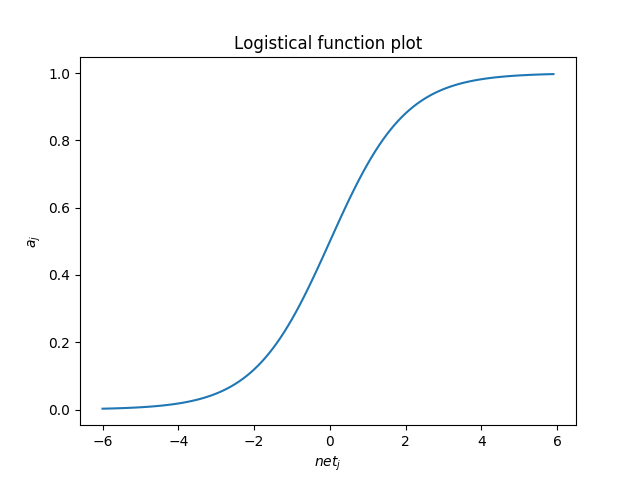
\includegraphics[scale=0.6]{10}
	\caption{Python plot for the logistic function}
\end{figure}

After the activation has been executed, the value of  $a_j$ is passed to the output function. The output function calculates the values to be distributed to the neurons whose inputs depend on this neuron’s output. For the neuron j, the output function of the neuron is:

\begin{equation}
	f_{out}=o_j	
\end{equation}

In the above equation, $o_j$ is the output of the output value of the neuron. Like the activation function, the output function is defined globally as well. In most cases, the output is the same as the value after the activation function:
\begin{align}
		f_{out}&=o_j \nonumber\\
	\text{But}\quad o_j&=a_j \nonumber\\
	\therefore f_{out}&=a_j
\end{align}

Different neural network topologies are analysed before making a choice on the correct implementation. Feedforward neural networks are the most trivial type of ANNs. The neurons that are in the network are divided into 3 layers. These layers are the input layer, the hidden layer and the output layer.

A plot of a simple feedforward neural network is shown below:
\begin{figure}[h]
	\centering
	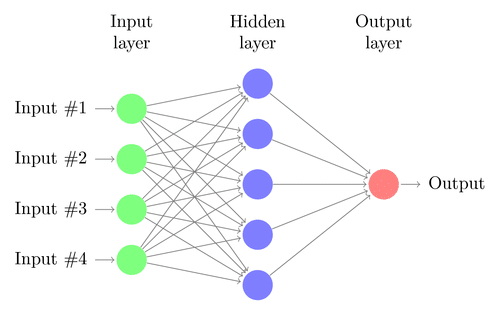
\includegraphics[scale=0.6]{11}
	\caption{Simple Neural Network with multiple input dependencies for each neuron}
\end{figure}

The neural network can have multiple hidden layers but only a single input layer as well as a single output layer. In this network topology, each layer’s neurons can only be directed to neurons in the next layer, thus the name feedforward network. Shortcut connections are possible for layers not immediately preceding the output layer to connect to the neurons at the output layer. A feedforward neural network works as follows: an input is supplied, and complex calculations are done on each neuron to produce final output values at the supposed output layer. However, there is an expected value associated with each input and the expected value is compared with the practical value output and the error associated with the result is calculated. This error is used to calculate the accuracy of the neural network.

There are different errors that can be used. Given output neurons are represented by $\Omega$ and the set representing output neurons is given by O, the specific error,$Err_p$ can be calculated by the equation:
\begin{equation}
	$\text { Err }$ _ { p } = \frac { 1 } { 2 } \sum_{ \Omega \in O }^{ }  \left( t _ { \Omega } - y _ { \Omega } \right) ^ { 2 }
\end{equation}

In the above neural network $t$ values are the true expected output values while $y$ values are the output values produced by the neural network. The Euclidean distance gives a more useful error value that the one calculated above as it will show how far the error correction has to be made to find the correct value. 
\begin{equation}
\operatorname {Err} _ { p } = \sqrt { \sum _ { \Omega \in O } \left( t _ { \Omega } - y _ { \Omega } \right) ^ { 2 } }
\end{equation}

The most desirable error is the root mean square error because it calculates the error values for the outlier outputs. This equation is shown below:
\begin{equation}
\operatorname { Err } _ { p } = \sqrt { \frac { \sum _ { \Omega \in O } \left( t _ { \Omega } - y _ { \Omega } \right) ^ { 2 } } { | O | } }
\end{equation}

The training of the neural network will follow an offline handwriting recognition scheme to minimize the learning time for the neural network. The outputs are batched and training occurs after a specific time period called an epoch. Epoch is an step in time where an expected value is calculated using feedforward propagation and the errors are corrected for weight adjustment for the dataset. The total error for each time interval of testing is important:

\begin{equation}
\text { Err } = \sum _ { p \in P } \operatorname { Err } _ { p }
\end{equation}

To be able to learn, the neural network uses a method called backpropagation where each neuron from the output back to the initial inputs has the weights of its inputs adjusted to minimize the error associated with the output. The gradient descent method is applied to the error. An example of the gradient descent is shown in the figure below:

\begin{figure}[h]
	\centering
	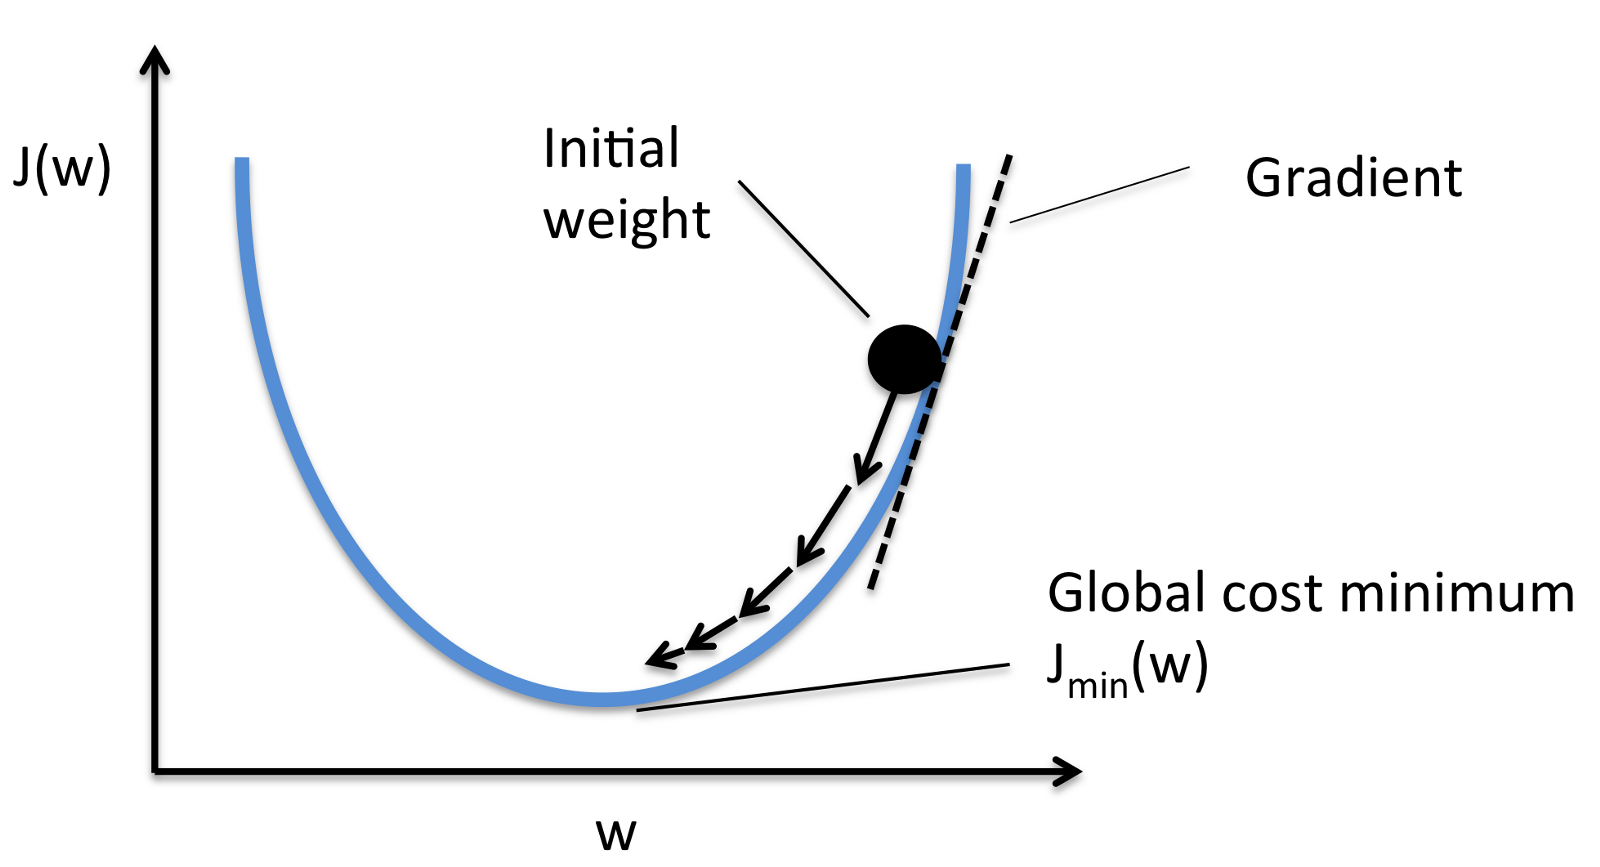
\includegraphics[scale=0.2]{31}
	\caption{Cost function example on which gradient descent can be applied.}
\end{figure}

The goal is to find a local minimum for each step so that the error is reduced to the minimum possible. The weight vector is gradually decreased, finding a new weight value that decreases the error function which is the cost function in the graph above. When the current position becomes the local minimum, instead of the one at the next step i.e. the net weight value increases the cost function instead of decreasing it, then mathematically the global minimum has been passed due to the step size being too large or the current value for the weight leads to the global minimum of the cost function. It is important to check the local minimum after every weight adjustment because continuous decrease without checking can overshoot the weight adjustment past the global minimum and weights end up a cost function that oscillates around the global cost minimum.

The neural network's learning function should model the figure that follows when  training data is supplied. The training data sample count does not have to be specific but the shape should follow or model the exponential curve. 

\begin{figure}[h]
	\centering
	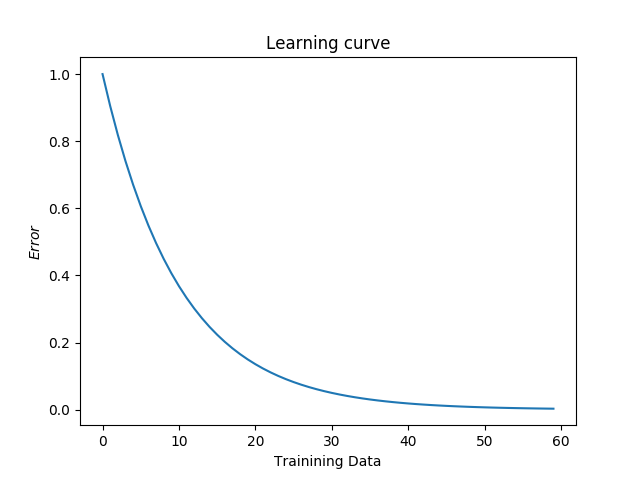
\includegraphics[scale=0.6]{30}
	\caption{Expected Learning curve for neural network}
\end{figure}

The value for adjusting the weights is directly proportional to the gradient of the cumulative Error.

\begin{align}
\Delta W \quad & \alpha \quad  \nabla \operatorname {Err} (W) \nonumber\\
\Delta W  &=  - \eta \nabla \operatorname { Err } ( W )
\end{align}
 
The constant $\eta$ is constant of proportionality known as the learning rate. It is equivalent to the step size of the weight adjustment. As described before, this value has to be optimized to avoid weight adjustments that lead to an oscillating error function. 

The gradient of the Error function is then expressed as the partial derivative with respect to the weights in the previous layer.
Every weight in the layer preceding the output layer is adjustment and the effect on the cumulative error function is analyzed. The adjustment follows the equation:

 \begin{equation}
 \Delta w _ { i , \Omega } = - \eta \frac { \partial \operatorname { Err } ( W ) } { \partial w _ { i , \Omega } }
  \end{equation}

The error function used for the weight adjustment is a combination of equation 3.17 and equation 3.19 so that:

\begin{align}
\text {Err}(W) &= \sum _ { p \in P } \operatorname { Err } _ { p }  \\
&= \sum_{p \in P} \big( \frac { 1 } { 2 } \sum _ { \Omega \in O } \left( t _ { \Omega } - y _ { \Omega } \right) ^ { 2 }\big)  \\
&=\frac{1}{2} \sum_{p \in P} \Big(  \sum _ { \Omega \in O } \left( t _ {p, \Omega } - y _ {p, \Omega } \right) ^ { 2 }\Big)
\end{align}

Equation 3.23 and 3.22 can be combined tp find the dependency of the weight ag=djustment on the individual errors:

\begin{align} 
	\Delta w _ { i , \Omega }  & = \sum _ { p \in P } - \eta \frac { \partial \operatorname { Err } _ { p } ( W ) } { \partial w _ { i , \Omega } } 
\end{align}

The partial derivative of each output's error function with respect to its weight is then calculated by using the chain rule so that the partial derivative of the error with respect to the ouput is multiplied by the partial derivative of the output with respect to the weight of that connection to the output.

\begin{equation}
\frac { \partial \operatorname { Err } _ { p } ( W ) } { \partial w _ { i , \Omega } } = \frac { \partial \operatorname { Err } _ { p } ( W ) } { \partial o _ { p , \Omega } } \cdot \frac { \partial o _ { p , \Omega } } { \partial w _ { i , \Omega } }
\end{equation}

The first argument of the equation in the chain rule can be broken down by first analyzing equation 3.17. This equation clearly shows that the error depends on the expected value of $t_{\Omega}$ and the observed value of $y_{\Omega}$. This value of $y_\Omega$ is the equivalent of the output value that is the derivative term i.e. $o_\Omega = y_\Omega$ as follows:
\begin{align}
\frac { \partial }{ \partial o _ { p , \Omega } }\Big(\operatorname { Err } _ { p } ( W )\Big) &= \frac { \partial }{ \partial o _ { p , \Omega } } \Big(\frac { 1 } { 2 } \sum _ { \Omega \in O } \left( t _ { \Omega } - o _ { \Omega } \right) ^ { 2 }\Big) \nonumber \\
&= (-1) \cdot 2 \cdot \frac{1}{2} \cdot (t_{p,\Omega} - o_{p,\Omega}) \nonumber \\
&= -(t_{p,\Omega} - o_{p,\Omega})
\end{align}

The specific error associated with the derivative can be replaced with a symbol $\delta_{p,\Omega} = t_{p, \Omega} - o_{p,\Omega}$. Equation 3.28 therefore becomes:
\begin{align}
\frac { \partial }{ \partial o _ { p , \Omega } }\Big(\operatorname { Err } _ { p } ( W )\Big) = -\delta_{p,\Omega}
\end{align}

Updating equation 3.27 leads to the equation:

\begin{align}
\frac { \partial \operatorname { Err } _ { p } ( W ) } { \partial w _ { i , \Omega } } &= \frac { \partial \operatorname { Err } _ { p } ( W ) } { \partial o _ { p , \Omega } } \cdot \frac { \partial o _ { p , \Omega } } { \partial w _ { i , \Omega } } \nonumber \\
 &= - \delta_{p,\Omega} \cdot \frac { \partial o _ { p , \Omega } } { \partial w _ { i , \Omega } }
\end{align}

For the derivative of the output with respect to the weight, it is realized that the output is the result after the activation process, which in turn depends on the net input as shown in equation 3.6 as this is a linear process as shown in Figure 9. This partial derivative reduces to:

\begin{align}
\frac { \partial o _ { p , \Omega } } { \partial w _ { i , \Omega } } &= \frac { \partial \sum _ { i \in I } \left( o _ { p , i } w _ { i , \Omega } \right) } { \partial w _ { i , \Omega } } \nonumber \\
\text{Therefore}\\
\frac { \partial \operatorname { Err } _ { p } ( W ) } { \partial w _ { i , \Omega } } &= - \delta _ { p , \Omega } \cdot \frac { \partial \sum _ { i \in I } \left( o _ { p , i } w _ { i , \Omega } \right) } { \partial w _ { i , \Omega } }
\end{align}

The above equation shows the summation of the outputs and th weights to destinations. However, all the derivatives are equal to 0 except for the term where the iterator $i=i$, sine they are constant with respect to $i$. The partial derivative of the output with respect to weight becomes:
\begin{align}
\frac { \partial o _ { p , \Omega } } { \partial w _ { i , \Omega } } &= \frac { \partial \sum _ { i \in I } \left( o _ { p , i } w _ { i , \Omega } \right) } { \partial w _ { i , \Omega } } \nonumber \\
&= \frac { \partial   \left( o _ { p , i } w _ { i , \Omega } \right) } { \partial w _ { i , \Omega } } \nonumber \\
&= o_{p,i}\\
\therefore \frac { \partial \operatorname { Err } _ { p } ( W ) } { \partial w _ { i , \Omega } } &= - \delta _ { p , \Omega } \cdot o_{p,i}
\end{align}

The equation (3.34) is inserted into the weight adjustment equation (3.26) to give the result:
\begin{align}
\Delta w _ { i , \Omega } &= \sum _ { p \in P } - \eta \frac { \partial \operatorname { Err } _ { p } ( W ) } { \partial w _ { i , \Omega } } \nonumber \\
&= \sum _ { p \in P } - \eta \cdot \big(- \delta _ { p , \Omega } \cdot o_{p,i}\big) \nonumber\\
&= \eta \sum _ { p \in P }   \delta _ { p , \Omega } \cdot o_{p,i}
\end{align}

The above equation will be the adjustment of the weight per epoch. To avoid the training time being too exponential, the training is done after every input which will be a screenshot of a line handwritten input. The equation then becomes:
\begin{align}
\Delta w _ { i , \Omega } &= \eta \cdot \delta _ { p , \Omega } \cdot o_{p,i}
\end{align}

Another type of neural network is the recurrent neural network. In general, for this type of network, each neuron contains a memory component that stores information about the previous input. In real life, when detecting a full sentence, the content of a word is dependent on the words detected before it. This type of neural network is therefore important in handwriting recognition. They are best applied to input that is only line segmented. A recurrent neural network works the same way as a feedforward network except the result for each input depends on the previous inputs. A recurring neural network consists of  multiple cascaded feedforward neural networks. The most important property of a recurring neural network is the presence of at least one feedback loop.

\begin{figure}[h]
	\centering
	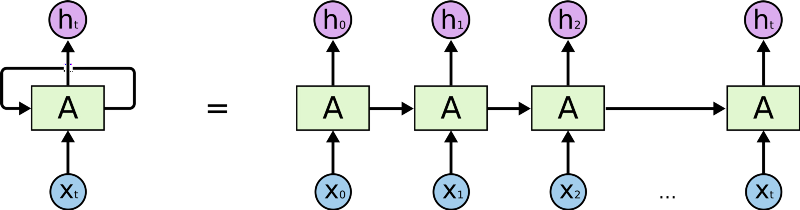
\includegraphics[scale=0.4]{12}
	\caption{Unfolding a Recurrent Neural Network}
\end{figure}

In the above example, for a time interval $t$, the $x_t$ values are the inputs, $A$ values are the neural network layers at time $t$ and $h_t$ values are the hidden state values at time $t$. The hidden state values from time $t-2$ or less are hidden from the state at time $t$ as it only has knowledge of the previous state. The output $h(t)$ is compared to the expected data output which is supplied in the test data. The error rate is calculated from this comparison and the backpropagation algorithm checks back to the previous layers of the neural network and adjusts the weights to minimize the error rate.\\
The present state can be summarized as being dependent on the current input and the parameters of the previous state:
\begin{align}
h _ { t } &= f _ { W } \left( h _ { t - 1 } , x _ { t } \right) \nonumber \\
h _ { t } &= \tanh \left( W _ { h h } h _ { t - 1 } + W _ { x h } x _ { t } \right)\nonumber\\
y _ { t } &= W _ { h y } h _ { t }
\end{align}

The equation above can be represented schematically by the diagram below:
\begin{figure}[h]
	\centering
	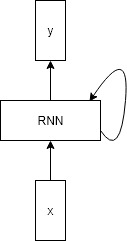
\includegraphics[scale=0.6]{15}
	\caption{Sketch showing the RNN process}
\end{figure}
\\
RNNs operate the same way as the previously described neural networks especially emphasizing on back propagation using the memory feature that they use. A problem arises where there is no stop condition due to the loop back being infinite and having no break condition. Learning could be done by unfolding the previous states of the RNN. The recurrences are backtracked, expanding the hidden states as shown in Figure 16. The earlier described backpropagation algorithm is applied to the unfolded Recurrent Neural Network. The weight values adjusted for RNNs from the backpropagation equations are the values of $W_{hh}$ and $W_{xh}$. Accuracy can be improved by expanding the non-output layers. The error associated with RNNs is dependent on the current and previous states i.e.
\begin{equation}
	Err_k = || \prod_{j=k+1}^{t} \frac{\partial h_j}{\partial h_{j-1}}||
\end{equation}

To prevent errors where the error associated with an input vanishes or disappears due to the exponential proportionality with time, Long Short Term Memory is used. Vanishing can occur if the product of the above equation keeps getting smaller with time while explosion occurs when the product exponentially increases.

The communication part of the device required the analysis of the GSM and well as the Wi-Fi method of communication. 
%If GSM were to be used for communication, the following diagram would model the architecture involved in the process.
\begin{figure}[h]
	\centering
	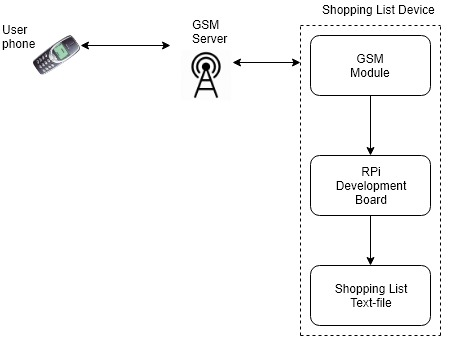
\includegraphics[scale=0.4]{17.jpg}
	\caption{Architecture involved in GSM communication}
\end{figure}

When GSM is used, mediums can communicate via voice or short message service or via fax. The operating frequencies of GSM communications are $450$ MHz, $800$ MHz, $900$ MHz, $1.8$ GHz and $2$ GHz. The operation associated with GSM communication is duplex. In Figure 15, the duplex operation is between the user phone and the GSM server. The frequency range for the cellphone to the GSM tower connection is called the uplink and the range for the server to the cellphone is called the downlink. Similarly, the uplink is the connection from the GSM module of the home shopping list device to the GSM tower. The connection from the GSM server to the home shopping list's GSM module is the downlink.\\
\begin{figure}[h]
	\centering
	
\includegraphics[scale=0.6]{17.png}
	\caption{User phone connection to the GSM tower}
\end{figure}

GSM architecture is divided into 3 layers:
\begin{itemize}
	\item Layer 1: Physical layer
	\item Layer 2: Data Link layer
	\item Layer 3: Network layer
\end{itemize}

The following diagram shows the connections of these layers between 2 devices communicating using GSM communication.
\begin{figure}[h]
	\centering
	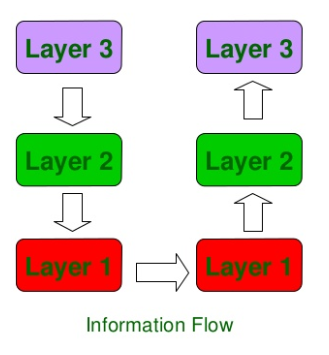
\includegraphics[scale=0.6]{24.png}
	\caption{Layer connections for GSM communication between 2 devices}
\end{figure} 

The network layer provides services to carry the message signal to its destination. The data link layer detects and resolves errors between the network layers of the 2 communicating devices. The physical layer i reponsible for transmission of the message signal on the physical medium. For example, a function like modulation for the transmission of data from the mobile station to the BTS occurs at the physical layer.

Each band is assigned a frequency by the GSM. This is known as Frequency Division Multiple Access.The size of each division is equal to 200 kHz.\\\\
The user's phone number on the service provider's network is known as the Mobile Subscriber ISDN. This is number is what is dialed by another subscriber to communicate with this subscriber. The MSISDN is split into  parts namely the Country Code represented by CC, the National Destination Code represented by NDC and the Subscriber Number represented by SN.\\
\begin{figure}[h]
	\centering
	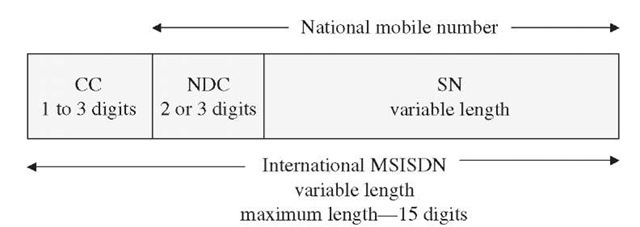
\includegraphics[scale=0.6]{20}
	\caption{MSISDN segments}
\end{figure}
\\
The CC is the international dialing code that the service provider of the subscriber is registered to. Each PLMN has its own NDC. The SN is the number that the user is registered as to the service provider. The concatenation of the NDC and the SN produces the National Mobile Number which is also known as the Local Mobile Number. This number is the nummber dialed by other subscribers in the same country as thee current user's service provider.\\
\begin{figure}[h]
	\centering
	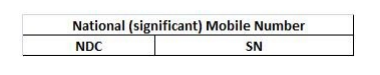
\includegraphics[scale=0.8]{21}
	\caption{National Mobile Number segments}
\end{figure}
\\
An example of a network provided by a service provider is the PLMN. The Mobile Station is subdivided into two modules: the Mobile Equipment represented by ME and the SIM.
\\
\begin{figure}[h]
	\centering
	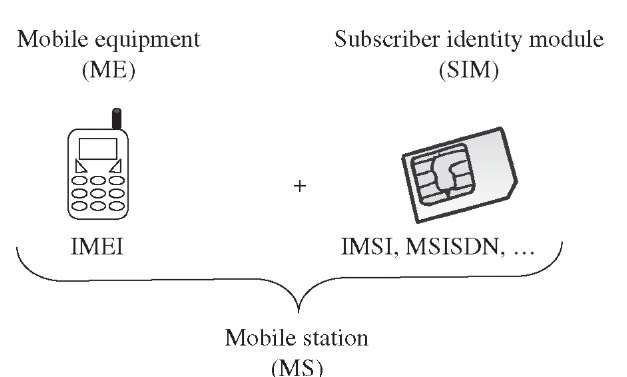
\includegraphics[scale=0.8]{22}
	\caption{A set-up of a Mobile Station}
\end{figure}
\\
As shown in the Figure 23, the ME is the physical component of the mobile station which is the cell phone. The primary requirement is that the phone should operate and communicate with other devices in a GSM network. The number of frequency bands that phones are operational in has increased from single to double to triple and finally to the modern phone which is quad-band. These phones have universal functionality in any GSM network. Each mobile handset has a unique International Mobile Equipment Identity printed onto it by the manufacturer.\\\\
The SIM is a very small card that should be inserted into the mobile phone for GSM connectivity. The card contains the subscriber's informations which includes their PIN code for access and the name of their service provider. The PIN code to access the SIM card is typically 4 digits long but if the code is entered wrongly for a certain amount of consecutive times depending on the service provider, the SIM cad is blocked. The user then has to enter an 8-digit PUK code to unblock the SIM card.

The model for the mobile station is adapted for the home shopping list device as well. Instead of the mobile equipment, the device can contain a GSM module integrated to the micro-controller that runs the shopping list device which is on the development board. The SIM card can then be placed inside the GSM module to form a fully functional mobile station.

The GSM network communicates with the mobile device or the shopping list device using a Base Transceiver Station. Multiple Base Transceiver Stations are controlled by a central Base Station Controller (BSC). The BSC also assigns radio frequencies from the mobile station.
\begin{figure}[h]
	\centering
	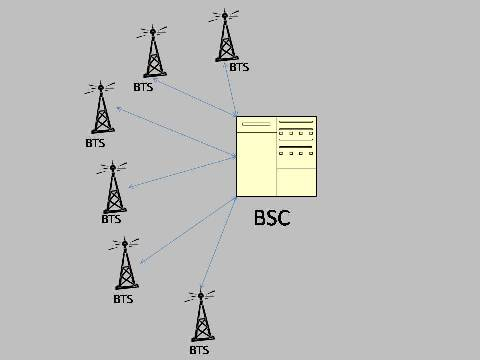
\includegraphics[scale=0.6]{23}
	\caption{BTS connections to a central BSC}
\end{figure}
\\
When the mobile station or the home shopping list device wants to access the GSM network, it goes through an authentication process which is normally at boot time, where the user has to prove their identity and be  permitted to use the network if they satisfy the authentication process. The authentication process is implemented by encryption. Cipher block design is used for development of the encryption algorithm. Some networks instead use convolutional coding for their encryption algorithms.

The central component of the GSM network is the Mobile Switching Center (MSC). The MSC handles the authentication process from the last paragraph. Calls are switched and mobile stations are granted roaming access using the Home Location Register (HLR) and the Visitor Location register. A mobile station's national mobile number is stored in the Equipment Identity Register (EIR) which has records of all mobile stations connected to the GSM network. The MSC can remotely access this EIR as can another MSC in a different mobile network.

Additionally a Short Message Service Centre is another component of the system and it stores holds transmitted messages into memory and sends them to the destination mobile stations. When a mobile station enters a different service provider's GSM network it can be granted access to services provided by this service provider at significantly higher than normal billing rates.

Interference is the most drawback associated with GSM communication. During a 2-way call, a user speaks for approximately half of the time as they spend approximately half of the time listening to the receiver[19]. Due to this property, the connection is made discontinuous leading to less power loss from each transmission. This works well for short message service as the communication does not need to be on all the time. 
 
Alternatively, Wi-Fi communication could be used. The theory associated with this communication method is discussed in the paragraphs that follow.
 
 
The IEEE 802.11 is the most widely used Wi-Fi standard. It is a standard of the Wireless Local Area Networks. The operating frequency bands of this protocol are typically $2.4$ GHz and $5$ GHz. The $5$ GHz spectrum provides more bandwidth, faster tranmsission speeds and higher reliability than the $2.4$ GHz frequency spectrum. Cell phones have undergone a gradual shift from circuit-switched networks ,which transmit data at peak speeds of 10 kbps to packet switched networks which transmit data at speeds of above 100 kbps. Wireless networks use packet switch for data transmission. The differences between packet switching and circuit switching are discussed in section 2.

WLAN was initially for operation in small-scale office rooms to avoid complex cabling in office computers. Therefore, most Wi-Fi systems extend to less than 200 m. The wireless networks can provide Internet access meaning communication is possible with devices beyond the radius as long as the sender is in the 200 m radius of the WLAN. Transmission speeds can go from 1 Mbps to as high as 10 Mbps [12]. 

What makes Wi-Fi more desirable than most communication models is that most modern devices come in with Wi-Fi functionality built-in just like GSM but the speed of transmission for WI-Fi is magnitudes of orders faster than GSM.

The basic topology of a Wi-Fi network is shown below.
\begin{figure}[h]
	\centering
	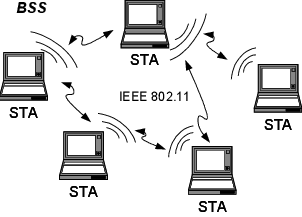
\includegraphics[scale=1]{25}
	\caption{Simple Wi-Fi topology for IBSS}
\end{figure}

For the above IBSS topology, the stations have peer-to-peer connections with each other and are called ad-hoc networks due to temporary connection style associated with the stations. These networks are very cheap and useful for tasks like conference meetings where user PCs only need connectivity with each other for a limited amount of time. This topology is extremely range limited. 

Multiple Basic Service Set topologies can be connected together by means of a distribution system to form an Extended Service Set topology. 
\begin{figure}[h]
	\centering
	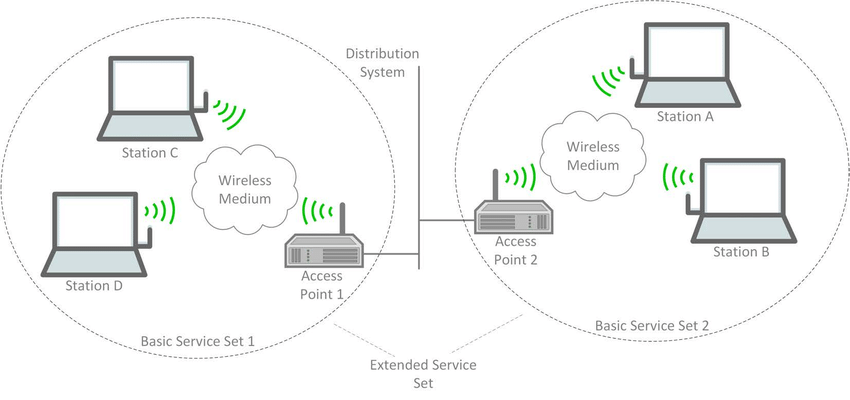
\includegraphics[scale=0.5]{26}
	\caption{Wi-Fi topology for ESS}
\end{figure}

The DS for the topology is usually any wireless network or Ethernet local area  network. The ESS enables the stations in different BSS networks to communicate with each other. The range available to ESS networks is significantly larger than the one provided by a single BSS topology. ESS is typically the design topology associated with Wi-Fi that covers entire university campuses.

The Access Point acts as a hub for wireless capable devices to communicate in the wireless LAN. The AP also authenticates devices that intend to devices that wish to communicate via the wireless network. The AP acts as the base station for PCs in the network. It also ports wireless networks together. A NIC is used by a a device with Wi-Fi capability for connectivity to the wireless network. The range of WLANs can be extended to kilometres by bridging LANs that are close to each other.


For the design of the Wi-Fi system, 3 design layouts were analyzed. A peer-to-peer wireless communication is when devices with NICs communicate directly with each other with no requirement for a server. The biggest problem with this layout is the range limit so a shopping list device with a NIC can only establish peer to peer connection with a user's phone when both devices are in the same residential range. Another layout is the Client and AP layout. The AP is connected to the service provider which offers server resources to the connecting PCs while extending their range of communication. The third layout is the Multiple AP layout. This is similar to the ESS topology where multiple APs are situated at different sites and they connect with each other to extend wireless coverage while giving wireless access to devices within their range.

A number of design limiting factors were analyzed for Wi-Fi. A device may have difficulty connecting to another AP in the ESS network. This can be due to to the connection not being therefore propagation delays being introduced and noise being introduced to the system through issues like interference. Peer to peer WLANs should only be used if the purpose is for the two device in the BSS to exclusively communicate with each other temporarily. The multiple AP WLANs should be used for devices who intend to access the Internet. The intended connection between the shopping list and the user's phone may use e-mail service for the shopping list device to receive a command to send the text and respond to the command with an email containing the text file. The use of the e-mail service implies the use of Internet therefore a multiple AP WLAN probably has to be implemented. However, peer-to-peer topology is used for the initial implementation of the WLAN. 

The interference of the WLAN can be due to other devices using frequency bands in the range similar to the one used for the WLANs i.e. $2.4$ GHz and $5$ GHz.  An example is the $2.4$ GHz 1EEE standard which competes with microwaves for frequency spectrum [22]. Due to this risk of interference, it is important for the information transmitted in the WLAN to be secured. Another big trade-off is that of battery life and bandwidth. The primary desire is data transmittion at high bandwidth but this leads to high battery drain for the Wi-Fi host. Therefore, for the home shopping list device an optimal frequency band has to be chosen so that battery drain is tolerable but not exponentially fast.  

The IEEE standard consists of 2 layers. These are Physical layer and the Media Acess control layer. The Physical layer consists of the frequency technology that is supported by the standard. These technolologies are frequency hopping, infrared and DS. Infrared technology is useful in BSS adhoc networks while microwave WLANs are used for multiple AP WLANs. DS WLANs need low traffic and transmit data at high data rates. The MAC layer is responsible for  the connection of the client device to the APs available. MAC also deals with the security of the WLAN.

The IEEE standards are split into 9 unique standards. The trade-off of interference for each standard is explored to choose the most applicable design. The important standards of note are:
\begin{itemize}
	\item 1EEE 802.11a : It is a physical layer standard which uses OFDM and priority is assigned to unique types of network traffic. The most important property is the low chance of interference due to operation in the $5$ GHz band. Transmission rates can be as high as 54 Mbps.
	\item IEEE 802.11b: Unlike the 802.11b standard, it operates in the $2.4$ GHz band and transmission speeds vary from 1 Mbps to 11 Mbps. Although the standard is old, other standards are just updates of this version with a few tweaks. The operation in the $2.4$ GHz band makes the standard susceptible to interference from other devices that operate in this frequency spectrum.
	\item IEEE 802.11c: This standard is important when designing and implementing access points so that APs can be bridged to extend WLAN coverage range.
	\item IEEE 802.11e: This standard is more dedicated to quality of service distribution for specific wireless local area networks. The standard focuses on the MAC layer to try to prioritize network traffic. Most of the priority is aimed at giving video and audio streaming services higher priority than the rest of the traffic. 
	\item IEEE 802.11f: When a Wi-Fi device switches between networks therefore switching to roaming mode, transmission packets are normally dropped and this standards atteempts to minimize the packets lost during handoffs when switching networks. Packets could also be dropped if an AP switches off due to some error and the device has to look for another AP in the multiple WLAN topology. 
	\item  IEEE 802.11g: The standard is backwards compatible with the 802.11b standard. It extends the transmission data rate of this protocol to be as high as 54 Mbps. Like the 802.11b standard,, the $2.4$ GHz band means the network is susceptible to interference as well.  
	\item IEEE 802.11i: This staandard focuses on the secure transfer of data on the network. All the other standards have weak security and this standard uses encryption for encryption schemes like AES to provide the best possible security.
\end{itemize}

Two stages are associated with each WLAN. These stages are authentication and encryption.
Authentication verifies if the client seeking communication is allowed to communicate with the server. Authentication can be provided by use of digital signatures or a pre-shared key.
The client has to prove they are who they claim to be. Encryption ensures secure data transfer between the two stations i.e. the user's phone and the home shopping list device. The data transferred over a wireless LAN can be susceptible to eavesdropping from hackers and the information transmitted can be compromised or worse, mal-ware can be attached to the file being transmitted. Examples of encryption schemes are Wired Equivalent Privacy and Wi-Fi Protected Access. WEP uses the same key at the client and the server for encryption and decryption.

The secure data transfer has to follow the stages shown in the diagram that follows.\\

\begin{figure}[h]
	\centering
	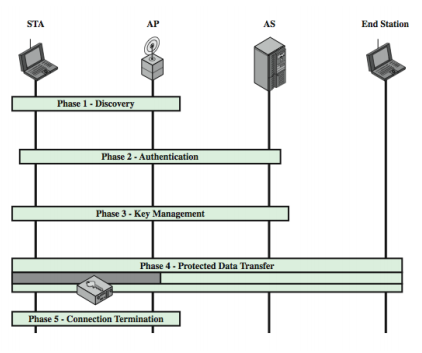
\includegraphics[scale=1]{28}
	\caption{Phases of operation for secure data transfer}
\end{figure}

The discovery phase involves the station and the access point identifying each other. The AP advertises its protocol using probe responses and the station detects them establishing an association between the two [17]. The authentication phase requires the station and the Authentication Server prove they are who they are to each other. Any data which is not for authentication is temporarily block from transmission in this phase. Cryptographic key generation is the next step in the phases shown and in the phase, the receiving stations receive these keys. If the communication is from one station to another via the use of an access point, like will be the case for the home shopping list to the user's phone, the keys will be group keys. If alternatively, the programmer intends to save the shopping list on the cloud which is on the Internet, then a pairwise key is generated for the AP. The two stations communicating can then exchange information between each other through the use of frames. Security is only applie to the station connection to the access point. Internet security can be implemented by using protocols like Secure Socket Layer protocol. E-mail already operates with SSL. After data exchange, the connection is terminated.

The comparison was also made between Wi-Fi and other wireless alternatives. Bluetooth transmission rates peak at  $\approx 800$ kpbs while Wi-Fi transmits at a significantly higher rate of $\approx 11$ Mbps. This project focuses on fast file transfer, therefore Wi-Fi is the more applicable choice for acceptable transmission times. If instead 3G communication is the alternative, then the decision for the right choice is a bit more close. The transmission speeds are a bit more closer as both schemes peak at $\approx 11$ Mbps. Wi-Fi is more design oriented for data transfer while 3G is an extension of the GSM communication with faster transfer rates. 

The home shopping device will be designed from different components with a development board. Most development boards are delivered with internal Wi-Fi modules while 3G modules have to purchased off the shelf and are fairly expensive. The 3G modules also have to be integrated onto the hardware which leads to either more wiring involved in the device if vero-boards are used or the device becoming larger in size which contradicts the requirement of the device being small-scale. Therefore for this project, Wi-Fi communication makes more sense to use as the data transmission method. 

\subsection{Modelling}

The handwriting writing and conversion process can be summarized by the flow chart below. The flow chart only documents the process from where the user writes onto the touchscreen until the user finishes writing onto the touchscreen.
\clearpage
\begin{figure}[h]
	\centering
	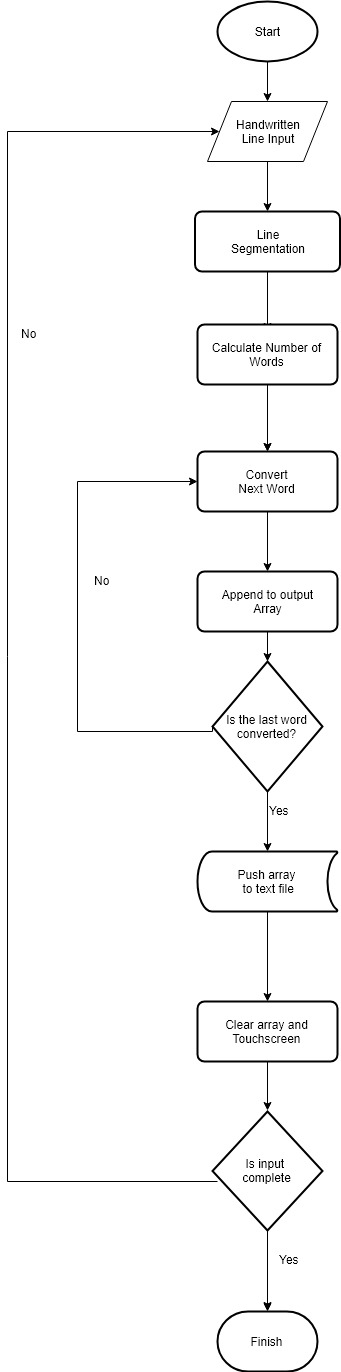
\includegraphics[scale=0.5]{34}
	\caption{Flowchart of the handwriting recognition process}
\end{figure}
\clearpage

A summary of the flow diagram is described. The user entered their shopping list line item onto the touchscreen. This input could be a sentence like "1 loaf of bread". The line input was only be restricted to one sentence per time and the sentence needed to be aligned on the touchscreen to reduce the skew. A line segmentation algorithm was applied to the input line so that the different words in the line could be obtained. In the sentence with, "1 loaf of bread", the words output after the line segmentation algorithm were "1", "loaf", "of" and "bread" separately. The number of these words was counted and the first word was converted. The converted output was pushed onto a string array. The word counter was reduced after successful word conversion and the word counter was checked if it was 0. If not, the next word was converted. After successful conversion, the output was appended with a space character between the initially converted word and the newly converted word. The word counter was decremented. The conversion process and appending the output onto an array was repeated until all the words from the line segmentation algorithm were completely converted. 

The output array after full conversion was then pushed to a text file and a new line was appended to the end of the text file sentence. The array containing the converted full word was then cleared to deallocate memory and the touchscreen was also cleared to provide input space for the net input. A button was made available for the user to indicate if they finished their input process.

Next, the shopping list from the conversion process had to be sent to the user's phone. The file had to be sent only when the user requested for it via e-mail. The flow chart on the next page details the steps that were taken for the file to be sent to the user's e-mail address. First, the Wi-Fi connection had to be established for the shopping list device to have an Internet connection. When an Internet connection had been established, the shopping list device would access the e-mail address assigned to it by default during the implementation process. The shopping list device would listen for a connection from the user's email address which was programmed within the communication algorithm. This process was generally known as the shopping device acting as the communicating server between the two devices, waiting for the client connection from the user's e-mail. When the user sent the e-mail, the sending process would be activated. The server was programmed to listen to any command from the user's email and this would trigger the process of sending the shopping list in the text file. The text file contents were read and stored  in an array of strings. The array of strings was then concatenated into a single string with elements separated by the newline character. The concatenated string was then sent to the user's email that had sent the command for the shopping list. The user then received the shopping list on their phone and did their shopping.
\clearpage
\begin{figure}[h]
	\centering
	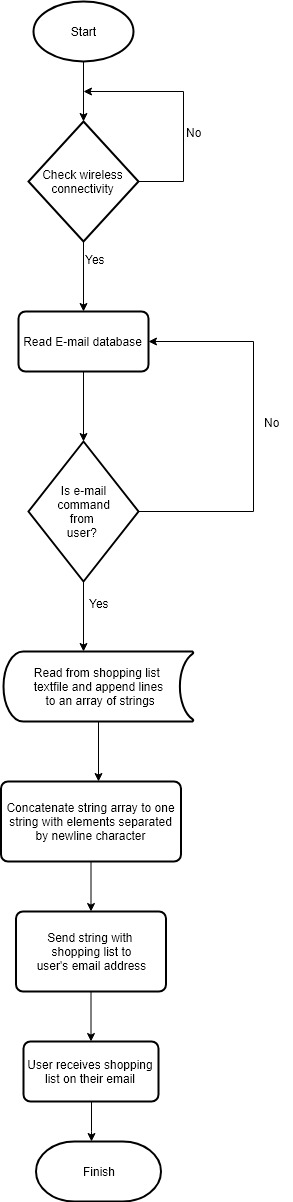
\includegraphics[scale=0.5]{36.jpg}
	\caption{Flowchart of sending the shopping list to the user's e-mail}
\end{figure}
\clearpage
\subsection{Optimization}
For the GSM network option, the transfer speeds of GSM are $\approx$ 10 kbps. The file size of the shopping list text file "shopping.txt" was found to be 586 kB. Therefore, the transmission time for the file to the user's device discounting the propagation delay was calculated as:
\begin{align*}
	t &= \frac{\text{File size}}{\text{Transmission Speed}}\\
	&= \frac{586 \times 8 \times 10^3 bits}{10 \times 10^3 bits/s}\\
	&= 46.9\,s
\end{align*}

This is way very slow and does not meet the time specifications of the product.

A trade-off is analyzed for the frequency band for the Wi-Fi communication. The frequency band in important in determining the Wi-Fi module to use for the shopping list device. Infrared waves cannot penetrate walls therefore are extremely range limited but offer very fast transmission speeds. On the other hand, radio waves can travel long distances but their data transmission rates are significantly lower. The two properties can be quantitatively compared by taking an example of 20 km between the source and destination. This models a situation where the customer shops 20 km from their home and requests the shopping the list in a wireless manner. The calculations associated with this transmission are shown below.\\
\newpage
\subsection{Data Design}
The software process of the project was modulated into different components. The components were listed as follows:
\begin{itemize}
	\item[1.]	Handwriting Recognition Algorithm
	\item[2.]	Graphical User Interface
	\item[3.]	E-mail communication
\end{itemize}

\textbf{Handwriting Recognition Algorithm}\\
The handwriting recognition algorithm was programmed using the Python programming language. Alternatively, it could be programmed by using Java, but the ability of Python to do mathematical functions on vectors was of great importance to reduce time complexity compared to Java which applied calculations element by element.

\textbf{Graphical User Interface}\\
The Graphical User Interface was programmed using PyQt, which uses the Python programming language for Widget development. PyQt was used instead of Qt because Qt uses the C++ environment, which complicates the integration process with the rest of the software components.

\textbf{E-mail Communication}\\
The e-mail communication software component facilitated the shopping list device receiving commands to send the shopping list and responding with the shopping list. Python programming was used for programming due to the availability of the Simple Mail Transfer Protocol which could be used to develop an e-mail server.

\subsubsection{Internal Software Data Structure}
The characteristic of the recognition algorithm to learn and update weight components required the use of  dynamic arrays. This is due to the fact that memory could be deallocated easily when dynamic arrays were used. Additionally, a 2-dimensional array will be associated with the PyQt GUI widget.

\subsubsection{Global Software Data Structure}
The output from the handwriting recognition process was saved globally so that it could be used by the e-mail server to send the shopping list to the client's phone therefore the string data structure, which was used to save the handwriting converted output was a global variable. Alternatively the data structure could have been a character array. Additionally, the shopping list could be requested any time, even during data input therefore the boolean data structure for listening to an incoming email request was global. 
\subsubsection{Temporary Data Structure}
The data structures which were temporary were mainly found in the recognition process. The errors were calculated for each output neuron and summed up before calculating the derivative. The error array then needed to be deallocated from memory. Another temporary variable was the count which was used for counting the number of words in the input sentence. As soon as the whole input was fully converted, this variable had to be reset and cleared until the next handwriting input. This variable was an integer.

\subsubsection{Database Description}
\textbf{2D Array Name}: widget$\_$Display\\
\textbf{Attributes}: save$\_$input, clear$\_$screen, capturedImage\\
\textbf{Description}: The array saved the resolution coordinates of the touchscreen and their colours. Initially, these were all zero values which represented the blank white screen. This database was important for the saving of user input by entering the non-white components of the touchscreen to their corresponding coordinates in the 2 dimensional array. The array contained integer values of  and 0, with 0 representing white and 1 representing non-white points from the screen-shot stored in capturedImage. \\\\
\textbf{2D Character Array Name}: shoppingList\\
\textbf{Attributes}: neural$\_$out, widget$\_$Display\\
\textbf{Description}: This array stored the outputs from the neural network. The neural network outputs were first concatenated after learning and error correction and they were then passed through a Viterbi algorithm to determine the closest word in the user's custom dictionary. The words were then combined to get the full initially input sentence. This word was then passed to the next free row of this array $shoppingList$ so that each row contained a sentence that was converted from the written sentence on the touchscreen, which was provided form widget$\_$Display.  \\\\
\textbf{Stack Name}: email$\_$Inbox\\
\textbf{Attributes}: email$\_$address, new$\_$mail\\
\textbf{Description}: The device had to access its email inbox database, first checking if new mail was received since the last access by using  the variable new$\_$mail which was a boolean. New mail was saved onto the argument stack and read. If the mail was not relevant, then the new$\_$mail variable would just be cleared but if the mail was from the desired client, the communication algorithm would send the shopping list to the email address of the stack element. 

\subsection{Architectural and Component Level Design}
\subsubsection{Program Description}
The structure chart method was used to represent the architectural diagram for the shopping list device. The dotted connections showed the partial dependencies of the architectural blocks connected. The classes that were designed to include the component block used the hierarchal class structure to show the most important classes for the device to be operational.
\subsubsection{Architecture Diagram}
The architectural block diagram of the home shopping list device software was shown below.
\begin{figure}[h]
	\centering
	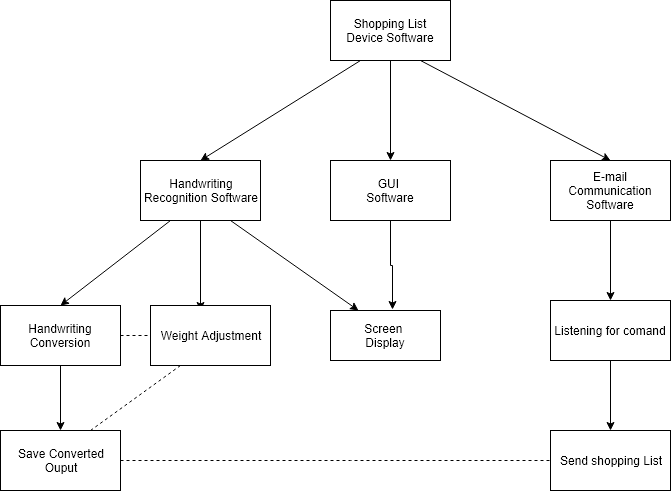
\includegraphics[scale=0.6]{38}
	\caption{Architectural diagram for the shopping list device}
\end{figure}

\subsubsection{Architectural Component Description}
The software component of the device was divided into 3 classes which were designed as shown in the figure that follows.
\begin{figure}[h]
	\centering
	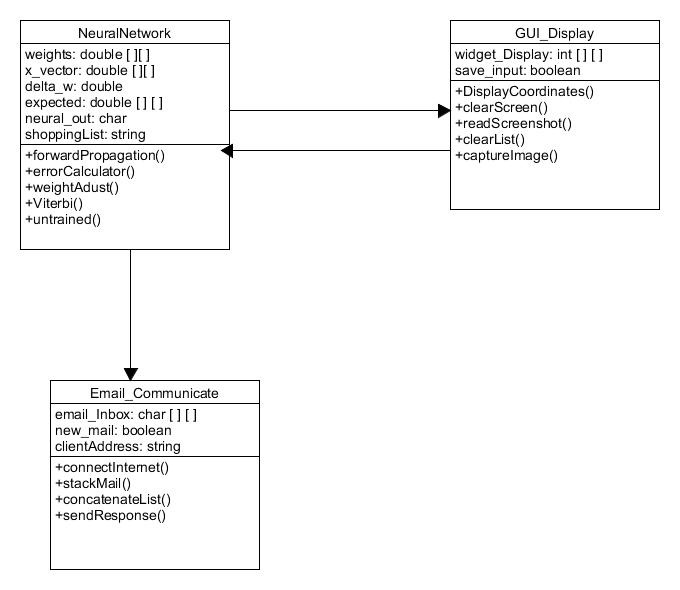
\includegraphics[scale=0.6]{42}
	\caption{Architectural diagram for the shopping list device}
\end{figure}

\subsubsection{Description of Components}
\textbf{Component NeuralNetwork}
\begin{itemize}
	\item \textbf{Processing Narrative of NeuralNetwork}: The attributes of the component include the weight matrix which was randomly generated, the input values from the touchscreen screen-shot, the character output after a neural network conversion and the full converted word. This was the most important component of the  home shopping list device's software because without it, no conversion would to take place thus the device would only contain handwritten screen-shots.
	\item \textbf{Interface Description of component NeuralNetwork}: The component interfaced with the GUI$\_$Display to get the vector representation of the 2D $x-$input array. It also saved the full word output to the full shopping list array which it passed to the communication component on request.
	\item \textbf{Algorithmic Description of the NeuralNetwork component}: The component links all three components of the software system as follows:\\
	\begin{itemize}
		\item[$\diamond$]	START
		\item[$\diamond$]	Get $\vec{x}$ from component GUI$\_$Display
		\item[$\diamond$]	Convert the full input sentence and store.
		\item[$\diamond$]	Listen for connection from Email$\_$Communicate and send the stored sentence. 
	\end{itemize}
\end{itemize}
The pseudocode for this component's most important function of handwriting recognition is shown below:
\begin{algorithmic}
	\STATE $\vec{x}$ $\Leftarrow$ GUI$\_$Procedure.widget$\_$Display 
	\STATE $\vec{w} \leftarrow$ \textbf{random}(length($\vec{x}$)) $\hfill \rightarrow$ Randommly generated weight array
	\STATE $x_{bias} = 1$  $\hfill \rightarrow$ Initialize bias neuron
	\STATE $w_{bias} = \textbf{random}$ $\hfill$ Generate weight of bias neuron
	\STATE $net_j = 0$ $\hfill$ Initialize neuron output
	\FOR {every neuron in every layer}
	\FOR {i in range length($\vec{x}$)}
		\STATE $net_j += \vec{x}\cdot vec{w}$
	\ENDFOR
	\STATE $net_j += x_{bias}\cdot w_{bias}$
	\STATE $a_j \leftarrow \frac{1}{1+e^{-net_j}}$
	\STATE $neuron_{out} \leftarrow a_j$
	\STATE $layer_out$ $\Leftarrow$ $neuron_out$
	\STATE Update $\vec{x}$ for next layer to consider $layer_{out}$
	\ENDFOR
	\IF {layer = outputLayer}
	\STATE$\sigma_s = neuron_{out} - e_j$ $\hfill$ Compare output to expected.
	\STATE $\Delta w = \sigma_s \cdot neuron_{out}$
	\WHILE {d ($\sigma_s$) $\neq 0$}
	\STATE $\vec{w} = \vec{w} - \Delta w$
	\STATE $net_j = \sum{\vec{w} \cdot \vec{x}} + 1\cdot (w_{bias})$
	\STATE$\sigma_s = neuron_{out} - e_j$  
	\ENDWHILE
		\STATE $output \leftarrow \frac{1}{1+e^{-net_j}}$
	\ENDIF
\end{algorithmic}

\textbf{Design  Class Hierarchy}\\
\begin{figure}[h]
	\centering
	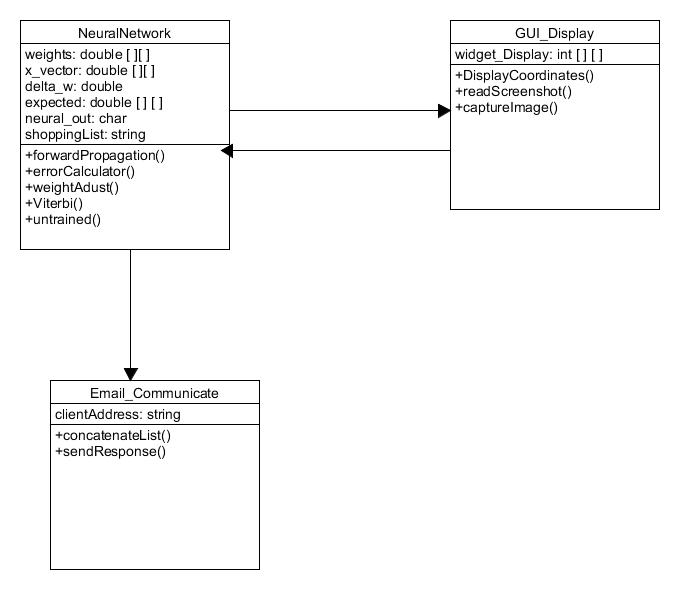
\includegraphics[scale=0.5]{41.jpg}
	\caption{Design class hierarchy for NeuralNetwork component}
\end{figure}

The design class hierarchy shows the specific functions from the connected functions that interact with the component.

\textbf{Restrictions}\\
 The number of hidden layers chosen had to be enough for significant accurate recognition but not too much because too much time would have been spent back-propagating and correcting errors.

\textbf{Component GUI$\_$Display}
\begin{itemize}
	\item \textbf{Processing Narrative of GUI$\_$Display}: The attributes in the component included the 2D array to save the equivalent screen inputs and a button which could clear the touchscreen when pressed.
	\item \textbf{Interface description of GUI$\_$Display}: The component interfaced with the NeuralNetwork component to provide the necessary vector array of inputs after converting the screen shot from the touchscreen to integer values in the array.
	\item \textbf{Algorithm Description of the GUI$\_$Display} : The link between the two components can be described in short as follows:
	\begin{itemize}
		\item[$\diamond$] START
		\item[$\diamond$] Prompt handwriting input
		\item[$\diamond$] Save Image of User Input
		\item[$\diamond$] Map the image coordinates to the 2D array of inputs.
	\end{itemize}
\end{itemize}
The pseudocode associated with the screen capturing and saving part is shown below:

\begin{algorithmic}
	\STATE widget$\_$Display = \textbf{empty}([] []) $\hfill$ Initialize empty GUI screen 
	\STATE coordinatesPen = [0,0] $\hfill$ Initialize mouse/pen drawing tool to null
	\IF {user enters drawing on screen}
	\WHILE {finishedDrawing $==$ \textbf{false}}
	\STATE draw += coordinatesPen $\hfill$ Take user's pen input.
	\ENDWHILE
	\STATE drawnImage = draw $\hfill$ The summed up user pen drawings.
	
	
	\textbf {for} {[\textbf{row}(drawnImage),\textbf{column}(drawnImage)]}  \textbf{do}
	\IF {drawnImage[row, column] == white}
	\STATE $widget\_Display$ [row, column] = 0
	\ELSE
	\STATE $widget\_Display$ [row, column] = 1
	\ENDIF
	
	\textbf{end for}
	%\ENDFOR
	
	\ENDIF 
\end{algorithmic}
	
\textbf{Design class hierarchy}
The design class hierarchy diagram shows the functions used by the NeuralNetwork component that interfaces with the GUI$\_$Display component.

\begin{figure}[h]
	\centering
	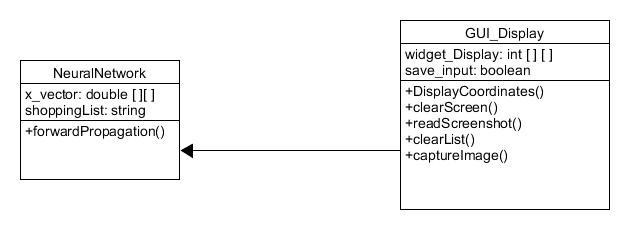
\includegraphics[scale=0.6]{43.jpg}
	\caption{Design class hierarchy for GUI$\_$Display component}
\end{figure}

\textbf{Restrictions}\\
The pen drawing application had a trade-off of fine ink which produced dots which overlapped against the pixel array but drawn characters were easily recognizable and sharp ink which produced the pen input images into different pixels but the image detection of the colours sometimes wrongly detected blank inputs due to the pixel most being white but containing a fraction of black ink.

\textbf{Component Email$\_$Communicate}
\begin{itemize}
	\item \textbf{Processing Narrative of Email$\_$Communicate}: The attributes in the component included the variable to check for new mail, the stack of inbox mail and the email address of the client
	\item  \textbf{Interface description of Email$\_$Communicate}: The component interfaced with the NeuralNetwork component to save the converted sentence into a string and store it as a text file offline. The file's contents would then be sent to the user's email address on request.
	\item \textbf{Algorithm Description of Email$\_$Communicate}: The tasks in volved in the component were shown procedurally as follows:
		\begin{itemize}
		\item[$\diamond$] START
		\item[$\diamond$] Update shopping list with new converted sentence.
		\item[$\diamond$] Check new mail and update onto mail stack.
		\item[$\diamond$] Check address of new mail.
		\item[$\diamond$] Send shopping list contents if the new mail email address is the same as the client address.
	\end{itemize}
\end{itemize}

\subsection{Design summary}
\begin{center}
	\begin{longtable}{|p{4cm}|p{7cm}|p{5cm}|}
		\hline 
		\textbf{Task} &
		\textbf{Implementation} &
		\textbf{Task Completion}
		\\
		\hline
		Design of non-USB battery system& The off the shelf 5 V battery was bought off the shelf. The Raspberry Pi's touchscreen and the Raspberry Pi were connected to it & Complete\\
		\hline
		&  &  \\
		\hline
		 &  & \\
		
		\hline
		\caption{Design summary.}
	\end{longtable}
\end{center}
\newpage

%% End of File.


%%
%%  Department of Electrical, Electronic and Computer Engineering.
%%  EPR400/2 Final Report - Section 4.
%%  Copyright (C) 2011-2018 University of Pretoria.
%%

\section{Results}

\subsection{Summary of results achieved}

\begin{center}
	\begin{longtable}{|p{5cm}|p{5cm}|p{5cm}|}
		\hline
		\textbf{Description of requirement or specification (intended outcome)} &
		\textbf{Actual outcome} &
		\textbf{Location in report} \\
		\hline 
		\multicolumn{3}{|l|} {\textbf{Mission requirements of the product}} \\
		\hline
		Text recognition should
		consider the probability of
		occurance of combinations of
		letters.
		&
		The Viterbi algorithm was successfully implemented to detect the closest words which were in the user's dictionary.
		&
		Section 4.2.1
		\\
		\hline
		The user should be able to undo an input onto the touchscreen and not have the written sentence converted to text.
		&
		The device's GUI had a "Clear" button which had the capability of resetting the touchscreen to being blank when clicked.
		&
		Section 4.2.3\\
		\hline
		The system should recognize
		that the user has completed
		writing their shopping list.
		& 
		The device's software system correctly realized when user input was finished by keeping track of the "Finished" button on the GUI, which when switched the booolean variable that tracked if input was finished.
		&  Section 4.2.3\\
		\hline
		\multicolumn{3}{|l|} {\textbf{Field Conditions}} \\
		\hline
		The device should read handwriting input from multiple users.
		&
		The device could accurately recognize handwritings from multiple users. 
		&
		Section 4.2.8
		\\
		\hline
		The device should operate under varying light conditions that will be typical of what the user will encounter in indoor environments.
		&
		Operation of the device was executed in a dark room and in the presence of a bright fluorescent light. The device successfully carried out all its function in the two different light conditions.
		&
		Section 4.2.11
		\\
		\hline
		\multicolumn{3}{|l|} {\textbf{Specifications}} \\
		\hline
		Information should be sent at
		request, to the mobile phone
		within 10 seconds.
		&
		The measured time for the transmission time of the email containing the shopping list was found to have a mean of 8.35 s
		&   
		Section 4.2.2
		\\
		\hline
		Accuracy of the handwriting
		character detection must be
		greater than 80$\%$.
		&
		The average accuracy calculated from different unseen handwritings was found to be 83.3$\%$.
		&   Section 4.2.1\\
		\hline
		The user must be warned
		when the battery power
		remaining is less than 10$\%$ of
		full capacity.
		&
		An algorithm was programmed to continuously check the battery progress bar as a global variable of the project and when it reached less than $10\%$, a boolean flag for low battery was triggered.
		&	Section 4.2.9\\
		\hline
		Handwritten input must be converted to text by the character recognition software in less than 1s.
		&
		The average conversion time for a line sentence input was measured to be 690 m s, using the timer. 
		&
		Section 4.2.3\\
		\hline
		The communication link
		between the device’s
		communication system
		and the phone system should
		transfer data bidirectionally,
		at a rate of between 5Mbps
		and 10Mbps so that the bit
		error rate can be less than
		10$\%$.
		&
		The Wi-Fi link on the device could communicate at speeds of 11 Mbps.
		&
		Section 4.2.2
		\\
		\hline
		\multicolumn{3}{|l|} {\textbf{Deliverables}} \\
		\hline
		Optical character recognition algorithm for handwritten input to text conversion. The algorithm will be implemented on the hand-held shopping list device.
		&
		The optical recognition algorithm was successfully designed for and implemented onto the software system.
		&
		Section 4.2.1
		\\
		\hline
		Integration of the embedded processor
		board, the communication system and the touchscreen LCD to make the shopping list hardware device.
		&
		The different hardware was integrated to create the full working physical system which could be attached to a fridge.
		&
		Section 4.2.6 \\
		\hline	
		\caption{Results summary}
	\end{longtable}

\end{center}

\subsection{Qualification tests}

\subsubsection{Qualification test 1: Measurement of handwriting recognition accuracy}

4.2.1.a Qualification test\\
\textit{Objectives of test / experiment}\\
The accuracy of the handwriting scheme was measured in the test. The converted output was also checked against the dictionary and the relevant output was shown.

\textit{Equipment used}\\
The Python programming language was used. The mathematical libraries contained as well as the tracking libraries were used to develop an algorithm that could keep track of the recognized outputs and compare them to the expected values. The pseudo-code for the Python program implemented to calculate the accuracy of the recognition algorithm is shown below:\\

\begin{algorithmic}
	\STATE expectedOuputs.txt $\Leftarrow$ $\hfill$ $\rightarrow$ Text file containing expected text outputs.
	\WHILE {userInput == \textbf{true}}  
	\STATE \textbf{getUserLineInput()}  \hfill $\rightarrow$ Capture the user's handwritten shopping list line.
	\STATE sentence $\leftarrow$ \textbf{convertLineInput()} \hfill $\rightarrow$ Save recognition output
	\STATE dictionaryOut $\leftarrow$ Viterbi(sentence) \hfill $\rightarrow$ Detect closest word in dictionary.
	\STATE shoppingList.txt $\leftarrow$ dictionaryOutput \hfill Append the shopping list with the recognized sentence.
	\ENDWHILE
	\STATE correct = 0 \hfill $\rightarrow$ Correctly recognized letters
	\STATE total = 0 \hfill $\rightarrow$ Total recognized letters.
	\FOR {every line in shoppingList.txt}
	\FOR {every character i in every line}
	\IF {shoppingList.i == expectOutputs.i}
	\STATE correct $\leftarrow$ correct++ \hfill Increment correct characters
	\ENDIF
	
	total $\leftarrow$ total$++$ \hfill Increment total detected characters
	\ENDFOR
	\ENDFOR
	
	\STATE accuracy  $=$ $\frac{\text{correct}}{\text{total}} \times 100\%$
\end{algorithmic}

\textit{Experimental Parameters and setup}\\
The above values of accuracy were the important test parameters and the algorithm was implemented in Python.

\textit{Experimental protocol}\\
The basic steps in the calculation of the accuracy were extracted from the comments in the pseudo-code above:
\begin{itemize}
	\item Take the user input and convert to the corresponding sentence.
	\item Take the sentence and convert its contents to relevant dictionary words.
	\item Compare every letter from this output to the expect shopping list contents.
	\item Calculate output value.
\end{itemize}

4.2.1.b Results and Observations\\\\
\textit{Measurements}
\begin{center}
	\begin{longtable}{|p{5cm}|p{5cm}|}
		\hline
		\textbf{Number of sentences} &
		\textbf{Average Accuracy ($\%$)} \\
		\hline
		5
		&
		92.5
		\\
		\hline
		10
		&
		88.76
		\\
		\hline
		15
		&
		81.95
		\\
		\hline
		20
		&
		78.32
		\\
		\hline
		30
		&
		82.81
		\\
		\hline
		\textbf{Cumulative accuracy}
		&
		84.87
		\\
		\hline		
		\caption{Accuracy results}
	\end{longtable}
\end{center}

\begin{figure}[h]
	\centering
	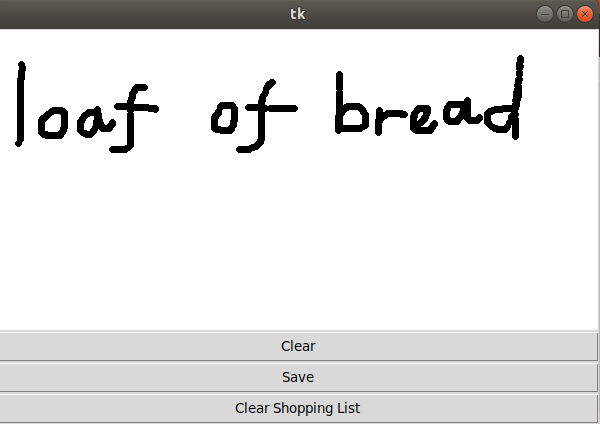
\includegraphics[scale=0.4]{101}
	\caption{First line user input}
\end{figure}

\begin{figure}[h]
	\centering
	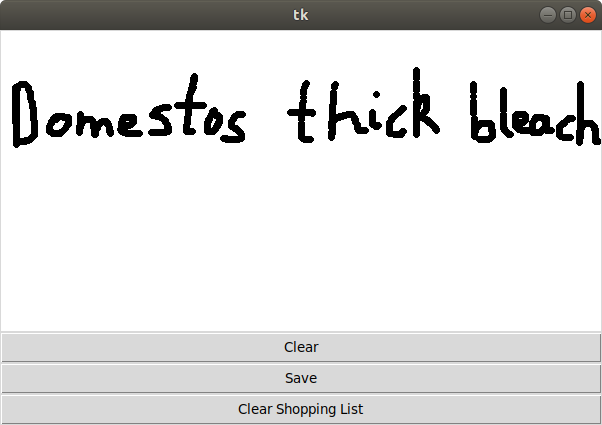
\includegraphics[scale=0.4]{102}
	\caption{Second line user input}
\end{figure}

\begin{figure}[h]
	\centering
	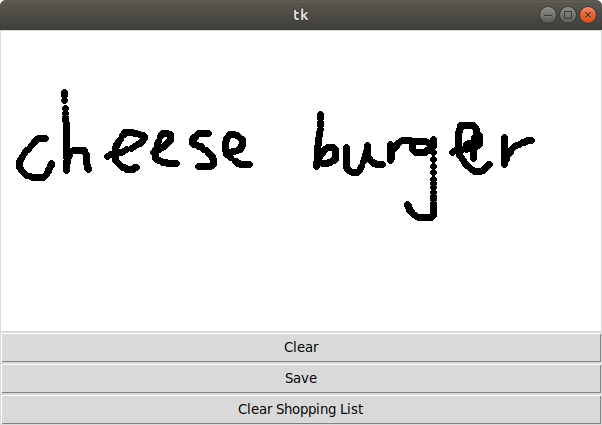
\includegraphics[scale=0.4]{103}
	\caption{Third line user input}
\end{figure}

\begin{figure}[h]
	\centering
	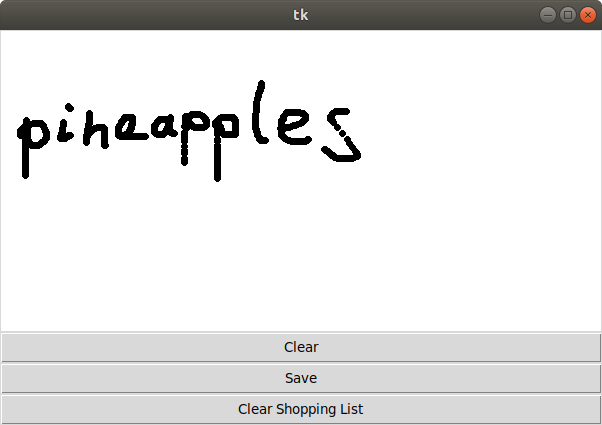
\includegraphics[scale=0.4]{105}
	\caption{Fifth line user input}
\end{figure}

\begin{figure}[h]
	\centering
	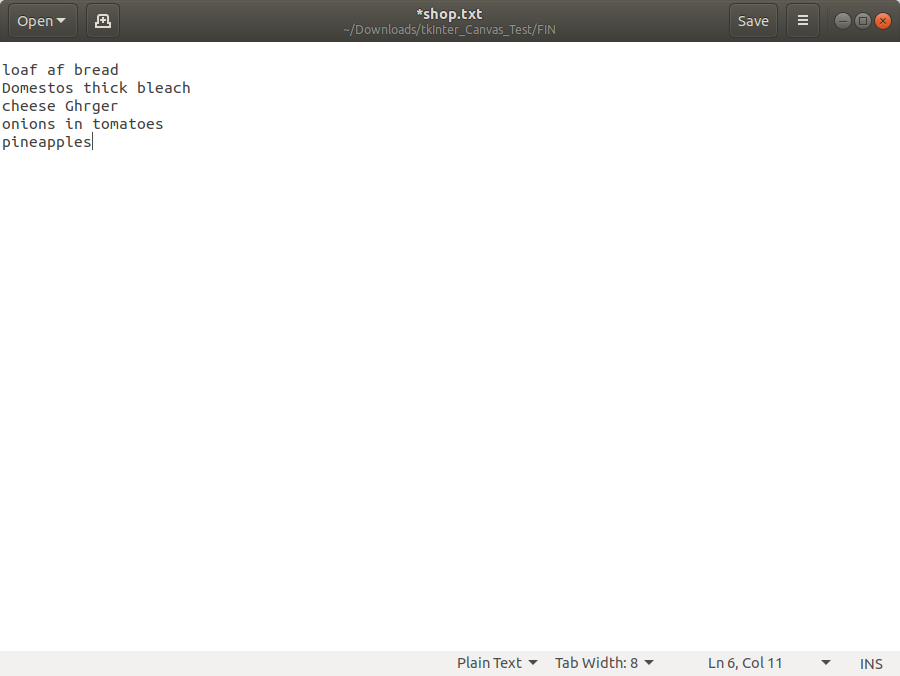
\includegraphics[scale=0.4]{106}
	\caption{Output text file containing shopping list}
\end{figure}
\clearpage
\textit{Description of results}\\
The accuracy of the recognition algorithm decreased as the number of sentences were doubled from 5 to 10. The accuracy decreased again as 5 more lines of user input were inserted. Addition of another 5 lines decreased the accuracy. Adding 10 more lines of user input led to an increase in the accuracy. The general accuracy was calculated to be 84.87$\%$

\subsubsection{Qualification test 2: Measurement of the transmission time for sending email}

4.2.2.a Qualification test\\
\textit{Objectives of test / experiment}\\
The time taken to send an email from the shopping list device to the user's email address. The wireless network's link capacity was also checked. 

\textit{Equipment used}\\
A Quartz stopwatch was used for timing.
\\

\textit{Experimental parameters and setup}\\
The value of $t_{transm}$ was the transmission time of note between the shopping list device sending the email and the message appearing on the user's inbox. The assumption was that the user had their e-mail service auto-refreshing at period of less than a second so that a new message was recognized immediately.

\textit{Experimental protocol}\\
The stages that were involved with the experiment were:
\begin{itemize}
	\item Reset the stopwatch to zero and open the email service on the user's phone.
	\item Run the mail algorithm code and simultaneously press the start button.
	\item Wait for the new email notification to pop up on the user's phone.
	\item  Stop the stopwatch when the email notification is observed by the user.
\end{itemize}

4.2.2.b Results and Observations\\
\textit{Measurements}\\
\begin{center}
	\begin{longtable}{|p{5cm}|p{5cm}|}
		\hline
		\textbf{File size (kiloBytes)} &
		\textbf{Transmission time (s)} \\
		\hline
		0.5
		&
		1.22
		\\
		\hline
		0.78
		&
		1.48
		\\
		\hline
		1.2
		&
		2.24
		\\
		\hline
		5.65
		&
		3.32
		\\
		\hline
		500
		&
		7.95
		\\
		\hline		
		\caption{Transmission time values.}
	\end{longtable}
\end{center}

\textit{Description of Results}\\
The first test was implemented for a file with 10 different sizes and of size 500 Bytes. The transmission time was extremely small. A few more lines were added and the transmission time was fast as well, only slower by a few hundredths of seconds. The lines of the text file were almost doubled and the transmission time increased by about a second. A bigger file i.e. an image was sent as the next argument and the transmission time was slower than the previous one by a second. A \textbf{.pdf} file was the file document sent by the e-mail system and although it was about 100 times larger than the previous file sent, it was only delivered in double the transmission time of the smaller file.

\subsubsection{Qualification test 3: System detection of user finishing handwriting process and handwriting conversion}

4.2.3.a Qualification test\\
\textit{Objectives of text / experiment}\\
The test involved the detection of the end of a user input process for their line sentence and the conversion of the line input in less than 1 second.

\textit{Equipment used}\\
The internal timing libraries of the Python environment were used. The Widget libraries were used to create GUI buttons which were kept track of by boolean variables. The pseudo-code for the conversion time calculation was shown below:\\

\begin{algorithmic}
	\STATE saveButton.clicked $\leftarrow$ \textbf{false} \hfill Initialize an unclicked button for save functionality  
	\WHILE {saveButton.clicked==\textbf{false}}
	\STATE drawn $\leftarrow$\textbf{false} userDrawing \hfill Model the input drawn
	\ENDWHILE
	\STATE $\rightarrow$ saveButton has now been clicked
	\STATE \textbf{startTimer()}
	\STATE convertInput \hfill $\rightarrow$ Apply Recognition algorithm
	\STATE \textbf{stopTimer()}
	\STATE $t_{reco}$ $\leftarrow$ timerValue	\hfill Recognition time value
\end{algorithmic}

\textit{Experimental Protocol}\\
The flow chart in Figure 36 shows the stages of the experimental protocol. 
\newpage
\begin{figure}[h]
	\centering
	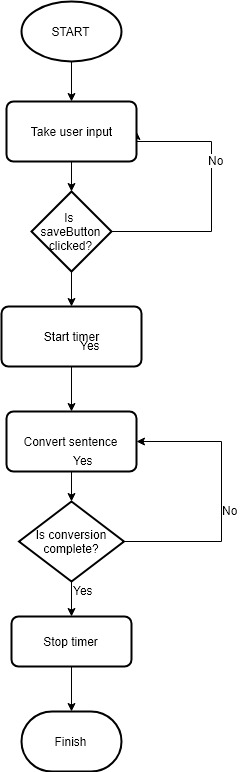
\includegraphics[scale=0.5]{50}
	\caption{Flow chart showing the experiment protocol}
\end{figure}

4.2.3.b Results and Observations\\
\textit{Measurements}\\
\begin{center}
	\begin{longtable}{|p{5cm}|p{5cm}|}
		\hline
		\textbf{Sentence number} &
		\textbf{Conversion time (s) ($\%$)} \\
		\hline
		1
		&
		0.43
		\\
		\hline
		2
		&
		0.88
		\\
		\hline
		3
		&
		0.32
		\\
		\hline
		4
		&
		0.65
		\\
		\hline
		5
		&
		0.49
		\\
		\hline
		\textbf{Average Conversion Time}
		&
		
		\\
		\hline		
		\caption{Accuracy results}
	\end{longtable}
\end{center}

\textit{Description of Results}\\

\newpage

%% End of File.



%%
%%  Department of Electrical, Electronic and Computer Engineering.
%%  EPR400/2 Final Report - Section 5.
%%  Copyright (C) 2011-2018 University of Pretoria.
%%

\section{Discussion}

%% ---[ BEGIN REMOVE ]---
{\slshape
Commence this section on a new page.

See the study guide -- this section is very important.  You need to show that
you can stand back and be critical of your own work. The worst possible thing
that you can write here is ``everything works perfectly''. There is no perfect
design, and you as (aspiring) engineer should be able to point out the
shortcomings of your design and/or results.

Tip: Use the headings in the study guide. These are not compulsory, but will
help you to organize your thoughts, and the headings actually tell you some of
the things that you are required to comment on.
}
%% ---[ END REMOVE ]---

\newpage

%% End of File.



%%
%%  Department of Electrical, Electronic and Computer Engineering.
%%  EPR400/2 Final Report - Section 6.
%%  Copyright (C) 2011-2018 University of Pretoria.
%%

\section{Conclusion}

%% ---[ BEGIN REMOVE ]---
{\slshape
Commence this section on a new page.
}
%% ---[ END REMOVE ]---

\subsection{Summary of the work}

%% ---[ BEGIN REMOVE ]---
{\slshape
Here you need to be extremely honest about what you achieved, and did not
achieve.

Conclusions need to be technical and MAY NOT relate to your personal
experience (e.g. ``I learnt a lot'' would be a good example of what NOT
to write).
}
%% ---[ END REMOVE ]---

\newpage

%% End of File.




%% Use the IEEE Transactions style for the references.
\bibliographystyle{IEEEtran}
\bibliography{finalreport}
\newpage

\newpage

%% --- PART 5 ------------------------------------------------------------

\eprsec{Part 5. Technical Documentation}

%%
%%  Department of Electrical, Electronic and Computer Engineering.
%%  EPR400/2 Final Report - Technical Documentation.
%%  Copyright (C) 2011-2018 University of Pretoria.
%%

\vspace*{0.5cm}

This main report is supplemented with technical documentation. This
provides more detail on the software that was used in the experiments,
including program listings, a user guide and circuit designs. This
section appears on the electronic media that accompanies this report.

The electronic media is organised into the directories listed below:
(give the directories as they appear on the electronic media).

{\itshape
Software \newline
References \newline
Datasheets \newline
Author \newline
Datasets/Raw \newline
Datasets/Final \newline
Project Photos \newline
Videos
}

%% End of File.



\newpage

\end{document}

%% End of File.
